\documentclass[a4paper, 92pt, twoside, openright]{report}
%% Fonts %%%%%%%%%%%%%%%%%%%%%%%%%%%%%%%%%%%%%%%%%%%%%%%%%%%%%%%%%%%%%%%%%%%%%
\usepackage[utf8]{inputenc}
\usepackage[T1]{fontenc}
\usepackage[english]{babel}
%\usepackage{lmodern} 
%\usepackage[upright]{fourier}
%\usepackage{ae,aecompl} 		% Utilisation des fontes vectorielles modernes
%\usepackage{amsmath}			% Permet de taper des formules mathématiques
%\usepackage{amssymb}			% Permet d'utiliser des symboles mathématiques
%\usepackage{amsfonts}			% Permet d'utiliser des polices mathématiques
%\usepackage{stmaryrd}
%\usepackage{nicefrac}			% Fractions 'inline'
% \usepackage[version=3]{mhchem}	% Equations chimiques
% \usepackage{arevmath}     		% For math symbols
\usepackage{xstring}

% Packages %%%%%%%%%%%%%%%%%%%%%%%%%%%%%%%%%%%%%%%%%%%
% \usepackage{xcolor,color, colortbl}
% \usepackage{pifont}
% \usepackage{eso-pic}
% \usepackage{anyfontsize}
% \usepackage{placeins}

% \usepackage{textcomp}
% \usepackage{hyphenat}
% \usepackage{import}
% \usepackage{pdfpages} 
\usepackage{multicol}
% \usepackage{wrapfig}
% \usepackage{float}
% \usepackage{etoolbox}
% \usepackage{adjustbox}
% \usepackage{siunitx}
% \usepackage{url}
% \usepackage{lscape,lipsum}
% \usepackage{everypage}
% \usepackage{eurosym}



%% Path %%%%%%%%%%%%%%%%%%%%%%%%%%%%%%%%%%%%%%%%%%%%%%%%%%%%%%%%%%%%%%%%%%%%%
\def\LIBPATH{../lib}
\def\REFPATH{../ref}
\def\RESPATH{../res}
\def\PLOTPATH{../res/plot}
\def\DATAPATH{../res/data}
\usepackage{xcolor,color, colortbl}

\definecolor{fondtitre}{rgb}{0.20,0.43,0.09}  % vert fonce
\definecolor{coultitre}{rgb}{0.41,0.05,0.05}  % marron
\definecolor{green}{rgb}{0.2,1,0.2}
\definecolor{beamer@blendedblue}{HTML}{404bbf}
\definecolor{violet}{HTML}{5c3566}
\definecolor{mygray}{rgb}{0.5,0.5,0.5}
\definecolor{mygreen}{rgb}{0,0.6,0}
\definecolor{gray75}{gray}{0.75}
\definecolor{marshalcolor}{rgb}{0.93,0.33,0.93} % MARSHAL blue
\definecolor{draftcolor}{rgb}{0.86,0.86,0.86} % MARSHAL draft color
\definecolor{darkraspberry}{rgb}{0.53, 0.15, 0.34}
\definecolor{darkgreen}{cmyk}{0.8,0,0.8,0.45}
\definecolor{lightgreen}{cmyk}{0.8,0,0.8,0.25}
%
\definecolor{mongris}{rgb}{0.5,0.5,0.5}
\definecolor{LightCyan}{rgb}{0.9,1,1}
\definecolor{DarkCyan}{rgb}{0.7,1,1}
\definecolor{LightGray}{gray}{0.5}
\definecolor{DarkGray}{gray}{0.85}
\definecolor{LightRed}{rgb}{1, 0.9, 0.9}
\definecolor{DarkRed}{rgb}{1, 0.8, 0.8}
\definecolor{mygreen}{rgb}{0,0.6,0}
\definecolor{mygray}{rgb}{0.5,0.5,0.5}
\definecolor{mymauve}{rgb}{0.58,0,0.82}
\definecolor{myred}{RGB}{220,43,25}
%\definecolor{mygreen}{RGB}{0,146,64}
\definecolor{myblue}{RGB}{0,143,224}
%
\definecolor{AliceBlue}{rgb}{0.94,0.97,1.00}
\definecolor{AntiqueWhite1}{rgb}{1.00,0.94,0.86}
\definecolor{AntiqueWhite2}{rgb}{0.93,0.87,0.80}
\definecolor{AntiqueWhite3}{rgb}{0.80,0.75,0.69}
\definecolor{AntiqueWhite4}{rgb}{0.55,0.51,0.47}
\definecolor{AntiqueWhite}{rgb}{0.98,0.92,0.84}
\definecolor{BlanchedAlmond}{rgb}{1.00,0.92,0.80}
\definecolor{BlueViolet}{rgb}{0.54,0.17,0.89}
\definecolor{CadetBlue1}{rgb}{0.60,0.96,1.00}
\definecolor{CadetBlue2}{rgb}{0.56,0.90,0.93}
\definecolor{CadetBlue3}{rgb}{0.48,0.77,0.80}
\definecolor{CadetBlue4}{rgb}{0.33,0.53,0.55}
\definecolor{CadetBlue}{rgb}{0.37,0.62,0.63}
\definecolor{CornflowerBlue}{rgb}{0.39,0.58,0.93}
\definecolor{DarkBlue}{rgb}{0.00,0.00,0.55}
\definecolor{DarkCyan}{rgb}{0.00,0.55,0.55}
\definecolor{DarkGoldenrod1}{rgb}{1.00,0.73,0.06}
\definecolor{DarkGoldenrod2}{rgb}{0.93,0.68,0.05}
\definecolor{DarkGoldenrod3}{rgb}{0.80,0.58,0.05}
\definecolor{DarkGoldenrod4}{rgb}{0.55,0.40,0.03}
\definecolor{DarkGoldenrod}{rgb}{0.72,0.53,0.04}
\definecolor{DarkGray}{rgb}{0.66,0.66,0.66}
\definecolor{DarkGreen}{rgb}{0.00,0.39,0.00}
\definecolor{DarkGrey}{rgb}{0.66,0.66,0.66}
\definecolor{DarkKhaki}{rgb}{0.74,0.72,0.42}
\definecolor{DarkMagenta}{rgb}{0.55,0.00,0.55}
\definecolor{DarkOliveGreen1}{rgb}{0.79,1.00,0.44}
\definecolor{DarkOliveGreen2}{rgb}{0.74,0.93,0.41}
\definecolor{DarkOliveGreen3}{rgb}{0.64,0.80,0.35}
\definecolor{DarkOliveGreen4}{rgb}{0.43,0.55,0.24}
\definecolor{DarkOliveGreen}{rgb}{0.33,0.42,0.18}
\definecolor{DarkOrange1}{rgb}{1.00,0.50,0.00}
\definecolor{DarkOrange2}{rgb}{0.93,0.46,0.00}
\definecolor{DarkOrange3}{rgb}{0.80,0.40,0.00}
\definecolor{DarkOrange4}{rgb}{0.55,0.27,0.00}
\definecolor{DarkOrange}{rgb}{1.00,0.55,0.00}
\definecolor{DarkOrchid1}{rgb}{0.75,0.24,1.00}
\definecolor{DarkOrchid2}{rgb}{0.70,0.23,0.93}
\definecolor{DarkOrchid3}{rgb}{0.60,0.20,0.80}
\definecolor{DarkOrchid4}{rgb}{0.41,0.13,0.55}
\definecolor{DarkOrchid}{rgb}{0.60,0.20,0.80}
\definecolor{DarkRed}{rgb}{0.55,0.00,0.00}
\definecolor{DarkSalmon}{rgb}{0.91,0.59,0.48}
\definecolor{DarkSeaGreen1}{rgb}{0.76,1.00,0.76}
\definecolor{DarkSeaGreen2}{rgb}{0.71,0.93,0.71}
\definecolor{DarkSeaGreen3}{rgb}{0.61,0.80,0.61}
\definecolor{DarkSeaGreen4}{rgb}{0.41,0.55,0.41}
\definecolor{DarkSeaGreen}{rgb}{0.56,0.74,0.56}
\definecolor{DarkSlateBlue}{rgb}{0.28,0.24,0.55}
\definecolor{DarkSlateGray1}{rgb}{0.59,1.00,1.00}
\definecolor{DarkSlateGray2}{rgb}{0.55,0.93,0.93}
\definecolor{DarkSlateGray3}{rgb}{0.47,0.80,0.80}
\definecolor{DarkSlateGray4}{rgb}{0.32,0.55,0.55}
\definecolor{DarkSlateGray}{rgb}{0.18,0.31,0.31}
\definecolor{DarkSlateGrey}{rgb}{0.18,0.31,0.31}
\definecolor{DarkTurquoise}{rgb}{0.00,0.81,0.82}
\definecolor{DarkViolet}{rgb}{0.58,0.00,0.83}
\definecolor{DeepPink1}{rgb}{1.00,0.08,0.58}
\definecolor{DeepPink2}{rgb}{0.93,0.07,0.54}
\definecolor{DeepPink3}{rgb}{0.80,0.06,0.46}
\definecolor{DeepPink4}{rgb}{0.55,0.04,0.31}
\definecolor{DeepPink}{rgb}{1.00,0.08,0.58}
\definecolor{DeepSkyBlue1}{rgb}{0.00,0.75,1.00}
\definecolor{DeepSkyBlue2}{rgb}{0.00,0.70,0.93}
\definecolor{DeepSkyBlue3}{rgb}{0.00,0.60,0.80}
\definecolor{DeepSkyBlue4}{rgb}{0.00,0.41,0.55}
\definecolor{DeepSkyBlue}{rgb}{0.00,0.75,1.00}
\definecolor{DimGray}{rgb}{0.41,0.41,0.41}
\definecolor{DimGrey}{rgb}{0.41,0.41,0.41}
\definecolor{DodgerBlue1}{rgb}{0.12,0.56,1.00}
\definecolor{DodgerBlue2}{rgb}{0.11,0.53,0.93}
\definecolor{DodgerBlue3}{rgb}{0.09,0.45,0.80}
\definecolor{DodgerBlue4}{rgb}{0.06,0.31,0.55}
\definecolor{DodgerBlue}{rgb}{0.12,0.56,1.00}
\definecolor{FloralWhite}{rgb}{1.00,0.98,0.94}
\definecolor{ForestGreen}{rgb}{0.13,0.55,0.13}
\definecolor{GhostWhite}{rgb}{0.97,0.97,1.00}
\definecolor{GreenYellow}{rgb}{0.68,1.00,0.18}
\definecolor{HotPink1}{rgb}{1.00,0.43,0.71}
\definecolor{HotPink2}{rgb}{0.93,0.42,0.65}
\definecolor{HotPink3}{rgb}{0.80,0.38,0.56}
\definecolor{HotPink4}{rgb}{0.55,0.23,0.38}
\definecolor{HotPink}{rgb}{1.00,0.41,0.71}
\definecolor{IndianRed1}{rgb}{1.00,0.42,0.42}
\definecolor{IndianRed2}{rgb}{0.93,0.39,0.39}
\definecolor{IndianRed3}{rgb}{0.80,0.33,0.33}
\definecolor{IndianRed4}{rgb}{0.55,0.23,0.23}
\definecolor{IndianRed}{rgb}{0.80,0.36,0.36}
\definecolor{LavenderBlush1}{rgb}{1.00,0.94,0.96}
\definecolor{LavenderBlush2}{rgb}{0.93,0.88,0.90}
\definecolor{LavenderBlush3}{rgb}{0.80,0.76,0.77}
\definecolor{LavenderBlush4}{rgb}{0.55,0.51,0.53}
\definecolor{LavenderBlush}{rgb}{1.00,0.94,0.96}
\definecolor{LawnGreen}{rgb}{0.49,0.99,0.00}
\definecolor{LemonChiffon1}{rgb}{1.00,0.98,0.80}
\definecolor{LemonChiffon2}{rgb}{0.93,0.91,0.75}
\definecolor{LemonChiffon3}{rgb}{0.80,0.79,0.65}
\definecolor{LemonChiffon4}{rgb}{0.55,0.54,0.44}
\definecolor{LemonChiffon}{rgb}{1.00,0.98,0.80}
\definecolor{LightBlue1}{rgb}{0.75,0.94,1.00}
\definecolor{LightBlue2}{rgb}{0.70,0.87,0.93}
\definecolor{LightBlue3}{rgb}{0.60,0.75,0.80}
\definecolor{LightBlue4}{rgb}{0.41,0.51,0.55}
\definecolor{LightBlue}{rgb}{0.68,0.85,0.90}
\definecolor{LightCoral}{rgb}{0.94,0.50,0.50}
\definecolor{LightCyan1}{rgb}{0.88,1.00,1.00}
\definecolor{LightCyan2}{rgb}{0.82,0.93,0.93}
\definecolor{LightCyan3}{rgb}{0.71,0.80,0.80}
\definecolor{LightCyan4}{rgb}{0.48,0.55,0.55}
\definecolor{LightCyan}{rgb}{0.88,1.00,1.00}
\definecolor{LightGoldenrod1}{rgb}{1.00,0.93,0.55}
\definecolor{LightGoldenrod2}{rgb}{0.93,0.86,0.51}
\definecolor{LightGoldenrod3}{rgb}{0.80,0.75,0.44}
\definecolor{LightGoldenrod4}{rgb}{0.55,0.51,0.30}
\definecolor{LightGoldenrodYellow}{rgb}{0.98,0.98,0.82}
\definecolor{LightGoldenrod}{rgb}{0.93,0.87,0.51}
\definecolor{LightGray}{rgb}{0.83,0.83,0.83}
\definecolor{LightGreen}{rgb}{0.56,0.93,0.56}
\definecolor{LightGrey}{rgb}{0.83,0.83,0.83}
\definecolor{LightPink1}{rgb}{1.00,0.68,0.73}
\definecolor{LightPink2}{rgb}{0.93,0.64,0.68}
\definecolor{LightPink3}{rgb}{0.80,0.55,0.58}
\definecolor{LightPink4}{rgb}{0.55,0.37,0.40}
\definecolor{LightPink}{rgb}{1.00,0.71,0.76}
\definecolor{LightSalmon1}{rgb}{1.00,0.63,0.48}
\definecolor{LightSalmon2}{rgb}{0.93,0.58,0.45}
\definecolor{LightSalmon3}{rgb}{0.80,0.51,0.38}
\definecolor{LightSalmon4}{rgb}{0.55,0.34,0.26}
\definecolor{LightSalmon}{rgb}{1.00,0.63,0.48}
\definecolor{LightSeaGreen}{rgb}{0.13,0.70,0.67}
\definecolor{LightSkyBlue1}{rgb}{0.69,0.89,1.00}
\definecolor{LightSkyBlue2}{rgb}{0.64,0.83,0.93}
\definecolor{LightSkyBlue3}{rgb}{0.55,0.71,0.80}
\definecolor{LightSkyBlue4}{rgb}{0.38,0.48,0.55}
\definecolor{LightSkyBlue}{rgb}{0.53,0.81,0.98}
\definecolor{LightSlateBlue}{rgb}{0.52,0.44,1.00}
\definecolor{LightSlateGray}{rgb}{0.47,0.53,0.60}
\definecolor{LightSlateGrey}{rgb}{0.47,0.53,0.60}
\definecolor{LightSteelBlue1}{rgb}{0.79,0.88,1.00}
\definecolor{LightSteelBlue2}{rgb}{0.74,0.82,0.93}
\definecolor{LightSteelBlue3}{rgb}{0.64,0.71,0.80}
\definecolor{LightSteelBlue4}{rgb}{0.43,0.48,0.55}
\definecolor{LightSteelBlue}{rgb}{0.69,0.77,0.87}
\definecolor{LightYellow1}{rgb}{1.00,1.00,0.88}
\definecolor{LightYellow2}{rgb}{0.93,0.93,0.82}
\definecolor{LightYellow3}{rgb}{0.80,0.80,0.71}
\definecolor{LightYellow4}{rgb}{0.55,0.55,0.48}
\definecolor{LightYellow}{rgb}{1.00,1.00,0.88}
\definecolor{LimeGreen}{rgb}{0.20,0.80,0.20}
\definecolor{MediumAquamarine}{rgb}{0.40,0.80,0.67}
\definecolor{MediumBlue}{rgb}{0.00,0.00,0.80}
\definecolor{MediumOrchid1}{rgb}{0.88,0.40,1.00}
\definecolor{MediumOrchid2}{rgb}{0.82,0.37,0.93}
\definecolor{MediumOrchid3}{rgb}{0.71,0.32,0.80}
\definecolor{MediumOrchid4}{rgb}{0.48,0.22,0.55}
\definecolor{MediumOrchid}{rgb}{0.73,0.33,0.83}
\definecolor{MediumPurple1}{rgb}{0.67,0.51,1.00}
\definecolor{MediumPurple2}{rgb}{0.62,0.47,0.93}
\definecolor{MediumPurple3}{rgb}{0.54,0.41,0.80}
\definecolor{MediumPurple4}{rgb}{0.36,0.28,0.55}
\definecolor{MediumPurple}{rgb}{0.58,0.44,0.86}
\definecolor{MediumSeaGreen}{rgb}{0.24,0.70,0.44}
\definecolor{MediumSlateBlue}{rgb}{0.48,0.41,0.93}
\definecolor{MediumSpringGreen}{rgb}{0.00,0.98,0.60}
\definecolor{MediumTurquoise}{rgb}{0.28,0.82,0.80}
\definecolor{MediumVioletRed}{rgb}{0.78,0.08,0.52}
\definecolor{MidnightBlue}{rgb}{0.10,0.10,0.44}
\definecolor{MintCream}{rgb}{0.96,1.00,0.98}
\definecolor{MistyRose1}{rgb}{1.00,0.89,0.88}
\definecolor{MistyRose2}{rgb}{0.93,0.84,0.82}
\definecolor{MistyRose3}{rgb}{0.80,0.72,0.71}
\definecolor{MistyRose4}{rgb}{0.55,0.49,0.48}
\definecolor{MistyRose}{rgb}{1.00,0.89,0.88}
\definecolor{NavajoWhite1}{rgb}{1.00,0.87,0.68}
\definecolor{NavajoWhite2}{rgb}{0.93,0.81,0.63}
\definecolor{NavajoWhite3}{rgb}{0.80,0.70,0.55}
\definecolor{NavajoWhite4}{rgb}{0.55,0.47,0.37}
\definecolor{NavajoWhite}{rgb}{1.00,0.87,0.68}
\definecolor{NavyBlue}{rgb}{0.00,0.00,0.50}
\definecolor{OldLace}{rgb}{0.99,0.96,0.90}
\definecolor{OliveDrab1}{rgb}{0.75,1.00,0.24}
\definecolor{OliveDrab2}{rgb}{0.70,0.93,0.23}
\definecolor{OliveDrab3}{rgb}{0.60,0.80,0.20}
\definecolor{OliveDrab4}{rgb}{0.41,0.55,0.13}
\definecolor{OliveDrab}{rgb}{0.42,0.56,0.14}
\definecolor{OrangeRed1}{rgb}{1.00,0.27,0.00}
\definecolor{OrangeRed2}{rgb}{0.93,0.25,0.00}
\definecolor{OrangeRed3}{rgb}{0.80,0.22,0.00}
\definecolor{OrangeRed4}{rgb}{0.55,0.15,0.00}
\definecolor{OrangeRed}{rgb}{1.00,0.27,0.00}
\definecolor{PaleGoldenrod}{rgb}{0.93,0.91,0.67}
\definecolor{PaleGreen1}{rgb}{0.60,1.00,0.60}
\definecolor{PaleGreen2}{rgb}{0.56,0.93,0.56}
\definecolor{PaleGreen3}{rgb}{0.49,0.80,0.49}
\definecolor{PaleGreen4}{rgb}{0.33,0.55,0.33}
\definecolor{PaleGreen}{rgb}{0.60,0.98,0.60}
\definecolor{PaleTurquoise1}{rgb}{0.73,1.00,1.00}
\definecolor{PaleTurquoise2}{rgb}{0.68,0.93,0.93}
\definecolor{PaleTurquoise3}{rgb}{0.59,0.80,0.80}
\definecolor{PaleTurquoise4}{rgb}{0.40,0.55,0.55}
\definecolor{PaleTurquoise}{rgb}{0.69,0.93,0.93}
\definecolor{PaleVioletRed1}{rgb}{1.00,0.51,0.67}
\definecolor{PaleVioletRed2}{rgb}{0.93,0.47,0.62}
\definecolor{PaleVioletRed3}{rgb}{0.80,0.41,0.54}
\definecolor{PaleVioletRed4}{rgb}{0.55,0.28,0.36}
\definecolor{PaleVioletRed}{rgb}{0.86,0.44,0.58}
\definecolor{PapayaWhip}{rgb}{1.00,0.94,0.84}
\definecolor{PeachPuff1}{rgb}{1.00,0.85,0.73}
\definecolor{PeachPuff2}{rgb}{0.93,0.80,0.68}
\definecolor{PeachPuff3}{rgb}{0.80,0.69,0.58}
\definecolor{PeachPuff4}{rgb}{0.55,0.47,0.40}
\definecolor{PeachPuff}{rgb}{1.00,0.85,0.73}
\definecolor{PowderBlue}{rgb}{0.69,0.88,0.90}
\definecolor{RosyBrown1}{rgb}{1.00,0.76,0.76}
\definecolor{RosyBrown2}{rgb}{0.93,0.71,0.71}
\definecolor{RosyBrown3}{rgb}{0.80,0.61,0.61}
\definecolor{RosyBrown4}{rgb}{0.55,0.41,0.41}
\definecolor{RosyBrown}{rgb}{0.74,0.56,0.56}
\definecolor{RoyalBlue1}{rgb}{0.28,0.46,1.00}
\definecolor{RoyalBlue2}{rgb}{0.26,0.43,0.93}
\definecolor{RoyalBlue3}{rgb}{0.23,0.37,0.80}
\definecolor{RoyalBlue4}{rgb}{0.15,0.25,0.55}
\definecolor{RoyalBlue}{rgb}{0.25,0.41,0.88}
\definecolor{SaddleBrown}{rgb}{0.55,0.27,0.07}
\definecolor{SandyBrown}{rgb}{0.96,0.64,0.38}
\definecolor{SeaGreen1}{rgb}{0.33,1.00,0.62}
\definecolor{SeaGreen2}{rgb}{0.31,0.93,0.58}
\definecolor{SeaGreen3}{rgb}{0.26,0.80,0.50}
\definecolor{SeaGreen4}{rgb}{0.18,0.55,0.34}
\definecolor{SeaGreen}{rgb}{0.18,0.55,0.34}
\definecolor{SkyBlue1}{rgb}{0.53,0.81,1.00}
\definecolor{SkyBlue2}{rgb}{0.49,0.75,0.93}
\definecolor{SkyBlue3}{rgb}{0.42,0.65,0.80}
\definecolor{SkyBlue4}{rgb}{0.29,0.44,0.55}
\definecolor{SkyBlue}{rgb}{0.53,0.81,0.92}
\definecolor{SlateBlue1}{rgb}{0.51,0.44,1.00}
\definecolor{SlateBlue2}{rgb}{0.48,0.40,0.93}
\definecolor{SlateBlue3}{rgb}{0.41,0.35,0.80}
\definecolor{SlateBlue4}{rgb}{0.28,0.24,0.55}
\definecolor{SlateBlue}{rgb}{0.42,0.35,0.80}
\definecolor{SlateGray1}{rgb}{0.78,0.89,1.00}
\definecolor{SlateGray2}{rgb}{0.73,0.83,0.93}
\definecolor{SlateGray3}{rgb}{0.62,0.71,0.80}
\definecolor{SlateGray4}{rgb}{0.42,0.48,0.55}
\definecolor{SlateGray}{rgb}{0.44,0.50,0.56}
\definecolor{SlateGrey}{rgb}{0.44,0.50,0.56}
\definecolor{SpringGreen1}{rgb}{0.00,1.00,0.50}
\definecolor{SpringGreen2}{rgb}{0.00,0.93,0.46}
\definecolor{SpringGreen3}{rgb}{0.00,0.80,0.40}
\definecolor{SpringGreen4}{rgb}{0.00,0.55,0.27}
\definecolor{SpringGreen}{rgb}{0.00,1.00,0.50}
\definecolor{SteelBlue1}{rgb}{0.39,0.72,1.00}
\definecolor{SteelBlue2}{rgb}{0.36,0.67,0.93}
\definecolor{SteelBlue3}{rgb}{0.31,0.58,0.80}
\definecolor{SteelBlue4}{rgb}{0.21,0.39,0.55}
\definecolor{SteelBlue}{rgb}{0.27,0.51,0.71}
\definecolor{VioletRed1}{rgb}{1.00,0.24,0.59}
\definecolor{VioletRed2}{rgb}{0.93,0.23,0.55}
\definecolor{VioletRed3}{rgb}{0.80,0.20,0.47}
\definecolor{VioletRed4}{rgb}{0.55,0.13,0.32}
\definecolor{VioletRed}{rgb}{0.82,0.13,0.56}
\definecolor{WhiteSmoke}{rgb}{0.96,0.96,0.96}
\definecolor{YellowGreen}{rgb}{0.60,0.80,0.20}
\definecolor{aliceblue}{rgb}{0.94,0.97,1.00}
\definecolor{antiquewhite}{rgb}{0.98,0.92,0.84}
\definecolor{aquamarine1}{rgb}{0.50,1.00,0.83}
\definecolor{aquamarine2}{rgb}{0.46,0.93,0.78}
\definecolor{aquamarine3}{rgb}{0.40,0.80,0.67}
\definecolor{aquamarine4}{rgb}{0.27,0.55,0.45}
\definecolor{aquamarine}{rgb}{0.50,1.00,0.83}
\definecolor{azure1}{rgb}{0.94,1.00,1.00}
\definecolor{azure2}{rgb}{0.88,0.93,0.93}
\definecolor{azure3}{rgb}{0.76,0.80,0.80}
\definecolor{azure4}{rgb}{0.51,0.55,0.55}
\definecolor{azure}{rgb}{0.94,1.00,1.00}
\definecolor{beige}{rgb}{0.96,0.96,0.86}
\definecolor{bisque1}{rgb}{1.00,0.89,0.77}
\definecolor{bisque2}{rgb}{0.93,0.84,0.72}
\definecolor{bisque3}{rgb}{0.80,0.72,0.62}
\definecolor{bisque4}{rgb}{0.55,0.49,0.42}
\definecolor{bisque}{rgb}{1.00,0.89,0.77}
\definecolor{black}{rgb}{0.00,0.00,0.00}
\definecolor{blanchedalmond}{rgb}{1.00,0.92,0.80}
\definecolor{blue1}{rgb}{0.00,0.00,1.00}
\definecolor{blue2}{rgb}{0.00,0.00,0.93}
\definecolor{blue3}{rgb}{0.00,0.00,0.80}
\definecolor{blue4}{rgb}{0.00,0.00,0.55}
\definecolor{blueviolet}{rgb}{0.54,0.17,0.89}
\definecolor{blue}{rgb}{0.00,0.00,1.00}
\definecolor{brown1}{rgb}{1.00,0.25,0.25}
\definecolor{brown2}{rgb}{0.93,0.23,0.23}
\definecolor{brown3}{rgb}{0.80,0.20,0.20}
\definecolor{brown4}{rgb}{0.55,0.14,0.14}
\definecolor{brown}{rgb}{0.65,0.16,0.16}
\definecolor{burlywood1}{rgb}{1.00,0.83,0.61}
\definecolor{burlywood2}{rgb}{0.93,0.77,0.57}
\definecolor{burlywood3}{rgb}{0.80,0.67,0.49}
\definecolor{burlywood4}{rgb}{0.55,0.45,0.33}
\definecolor{burlywood}{rgb}{0.87,0.72,0.53}
\definecolor{cadetblue}{rgb}{0.37,0.62,0.63}
\definecolor{chartreuse1}{rgb}{0.50,1.00,0.00}
\definecolor{chartreuse2}{rgb}{0.46,0.93,0.00}
\definecolor{chartreuse3}{rgb}{0.40,0.80,0.00}
\definecolor{chartreuse4}{rgb}{0.27,0.55,0.00}
\definecolor{chartreuse}{rgb}{0.50,1.00,0.00}
\definecolor{chocolate1}{rgb}{1.00,0.50,0.14}
\definecolor{chocolate2}{rgb}{0.93,0.46,0.13}
\definecolor{chocolate3}{rgb}{0.80,0.40,0.11}
\definecolor{chocolate4}{rgb}{0.55,0.27,0.07}
\definecolor{chocolate}{rgb}{0.82,0.41,0.12}
\definecolor{coral1}{rgb}{1.00,0.45,0.34}
\definecolor{coral2}{rgb}{0.93,0.42,0.31}
\definecolor{coral3}{rgb}{0.80,0.36,0.27}
\definecolor{coral4}{rgb}{0.55,0.24,0.18}
\definecolor{coral}{rgb}{1.00,0.50,0.31}
\definecolor{cornflowerblue}{rgb}{0.39,0.58,0.93}
\definecolor{cornsilk1}{rgb}{1.00,0.97,0.86}
\definecolor{cornsilk2}{rgb}{0.93,0.91,0.80}
\definecolor{cornsilk3}{rgb}{0.80,0.78,0.69}
\definecolor{cornsilk4}{rgb}{0.55,0.53,0.47}
\definecolor{cornsilk}{rgb}{1.00,0.97,0.86}
\definecolor{cyan1}{rgb}{0.00,1.00,1.00}
\definecolor{cyan2}{rgb}{0.00,0.93,0.93}
\definecolor{cyan3}{rgb}{0.00,0.80,0.80}
\definecolor{cyan4}{rgb}{0.00,0.55,0.55}
\definecolor{cyan}{rgb}{0.00,1.00,1.00}
\definecolor{darkblue}{rgb}{0.00,0.00,0.55}
\definecolor{darkcyan}{rgb}{0.00,0.55,0.55}
\definecolor{darkgoldenrod}{rgb}{0.72,0.53,0.04}
\definecolor{darkgray}{rgb}{0.66,0.66,0.66}
\definecolor{darkgreen}{rgb}{0.00,0.39,0.00}
\definecolor{darkgrey}{rgb}{0.66,0.66,0.66}
\definecolor{darkkhaki}{rgb}{0.74,0.72,0.42}
\definecolor{darkmagenta}{rgb}{0.55,0.00,0.55}
\definecolor{darkolive}{rgb}{0.33,0.42,0.18}
\definecolor{darkorange}{rgb}{1.00,0.55,0.00}
\definecolor{darkorchid}{rgb}{0.60,0.20,0.80}
\definecolor{darkred}{rgb}{0.55,0.00,0.00}
\definecolor{darksalmon}{rgb}{0.91,0.59,0.48}
\definecolor{darksea}{rgb}{0.56,0.74,0.56}
\definecolor{darkslate}{rgb}{0.18,0.31,0.31}
\definecolor{darkslate}{rgb}{0.18,0.31,0.31}
\definecolor{darkslate}{rgb}{0.28,0.24,0.55}
\definecolor{darkturquoise}{rgb}{0.00,0.81,0.82}
\definecolor{darkviolet}{rgb}{0.58,0.00,0.83}
\definecolor{deeppink}{rgb}{1.00,0.08,0.58}
\definecolor{deepsky}{rgb}{0.00,0.75,1.00}
\definecolor{dimgray}{rgb}{0.41,0.41,0.41}
\definecolor{dimgrey}{rgb}{0.41,0.41,0.41}
\definecolor{dodgerblue}{rgb}{0.12,0.56,1.00}
\definecolor{firebrick1}{rgb}{1.00,0.19,0.19}
\definecolor{firebrick2}{rgb}{0.93,0.17,0.17}
\definecolor{firebrick3}{rgb}{0.80,0.15,0.15}
\definecolor{firebrick4}{rgb}{0.55,0.10,0.10}
\definecolor{firebrick}{rgb}{0.70,0.13,0.13}
\definecolor{floralwhite}{rgb}{1.00,0.98,0.94}
\definecolor{forestgreen}{rgb}{0.13,0.55,0.13}
\definecolor{gainsboro}{rgb}{0.86,0.86,0.86}
\definecolor{ghostwhite}{rgb}{0.97,0.97,1.00}
\definecolor{gold1}{rgb}{1.00,0.84,0.00}
\definecolor{gold2}{rgb}{0.93,0.79,0.00}
\definecolor{gold3}{rgb}{0.80,0.68,0.00}
\definecolor{gold4}{rgb}{0.55,0.46,0.00}
\definecolor{goldenrod1}{rgb}{1.00,0.76,0.15}
\definecolor{goldenrod2}{rgb}{0.93,0.71,0.13}
\definecolor{goldenrod3}{rgb}{0.80,0.61,0.11}
\definecolor{goldenrod4}{rgb}{0.55,0.41,0.08}
\definecolor{goldenrod}{rgb}{0.85,0.65,0.13}
\definecolor{gold}{rgb}{1.00,0.84,0.00}
\definecolor{gray0}{rgb}{0.00,0.00,0.00}
\definecolor{gray100}{rgb}{1.00,1.00,1.00}
\definecolor{gray10}{rgb}{0.10,0.10,0.10}
\definecolor{gray11}{rgb}{0.11,0.11,0.11}
\definecolor{gray12}{rgb}{0.12,0.12,0.12}
\definecolor{gray13}{rgb}{0.13,0.13,0.13}
\definecolor{gray14}{rgb}{0.14,0.14,0.14}
\definecolor{gray15}{rgb}{0.15,0.15,0.15}
\definecolor{gray16}{rgb}{0.16,0.16,0.16}
\definecolor{gray17}{rgb}{0.17,0.17,0.17}
\definecolor{gray18}{rgb}{0.18,0.18,0.18}
\definecolor{gray19}{rgb}{0.19,0.19,0.19}
\definecolor{gray1}{rgb}{0.01,0.01,0.01}
\definecolor{gray20}{rgb}{0.20,0.20,0.20}
\definecolor{gray21}{rgb}{0.21,0.21,0.21}
\definecolor{gray22}{rgb}{0.22,0.22,0.22}
\definecolor{gray23}{rgb}{0.23,0.23,0.23}
\definecolor{gray24}{rgb}{0.24,0.24,0.24}
\definecolor{gray25}{rgb}{0.25,0.25,0.25}
\definecolor{gray26}{rgb}{0.26,0.26,0.26}
\definecolor{gray27}{rgb}{0.27,0.27,0.27}
\definecolor{gray28}{rgb}{0.28,0.28,0.28}
\definecolor{gray29}{rgb}{0.29,0.29,0.29}
\definecolor{gray2}{rgb}{0.02,0.02,0.02}
\definecolor{gray30}{rgb}{0.30,0.30,0.30}
\definecolor{gray31}{rgb}{0.31,0.31,0.31}
\definecolor{gray32}{rgb}{0.32,0.32,0.32}
\definecolor{gray33}{rgb}{0.33,0.33,0.33}
\definecolor{gray34}{rgb}{0.34,0.34,0.34}
\definecolor{gray35}{rgb}{0.35,0.35,0.35}
\definecolor{gray36}{rgb}{0.36,0.36,0.36}
\definecolor{gray37}{rgb}{0.37,0.37,0.37}
\definecolor{gray38}{rgb}{0.38,0.38,0.38}
\definecolor{gray39}{rgb}{0.39,0.39,0.39}
\definecolor{gray3}{rgb}{0.03,0.03,0.03}
\definecolor{gray40}{rgb}{0.40,0.40,0.40}
\definecolor{gray41}{rgb}{0.41,0.41,0.41}
\definecolor{gray42}{rgb}{0.42,0.42,0.42}
\definecolor{gray43}{rgb}{0.43,0.43,0.43}
\definecolor{gray44}{rgb}{0.44,0.44,0.44}
\definecolor{gray45}{rgb}{0.45,0.45,0.45}
\definecolor{gray46}{rgb}{0.46,0.46,0.46}
\definecolor{gray47}{rgb}{0.47,0.47,0.47}
\definecolor{gray48}{rgb}{0.48,0.48,0.48}
\definecolor{gray49}{rgb}{0.49,0.49,0.49}
\definecolor{gray4}{rgb}{0.04,0.04,0.04}
\definecolor{gray50}{rgb}{0.50,0.50,0.50}
\definecolor{gray51}{rgb}{0.51,0.51,0.51}
\definecolor{gray52}{rgb}{0.52,0.52,0.52}
\definecolor{gray53}{rgb}{0.53,0.53,0.53}
\definecolor{gray54}{rgb}{0.54,0.54,0.54}
\definecolor{gray55}{rgb}{0.55,0.55,0.55}
\definecolor{gray56}{rgb}{0.56,0.56,0.56}
\definecolor{gray57}{rgb}{0.57,0.57,0.57}
\definecolor{gray58}{rgb}{0.58,0.58,0.58}
\definecolor{gray59}{rgb}{0.59,0.59,0.59}
\definecolor{gray5}{rgb}{0.05,0.05,0.05}
\definecolor{gray60}{rgb}{0.60,0.60,0.60}
\definecolor{gray61}{rgb}{0.61,0.61,0.61}
\definecolor{gray62}{rgb}{0.62,0.62,0.62}
\definecolor{gray63}{rgb}{0.63,0.63,0.63}
\definecolor{gray64}{rgb}{0.64,0.64,0.64}
\definecolor{gray65}{rgb}{0.65,0.65,0.65}
\definecolor{gray66}{rgb}{0.66,0.66,0.66}
\definecolor{gray67}{rgb}{0.67,0.67,0.67}
\definecolor{gray68}{rgb}{0.68,0.68,0.68}
\definecolor{gray69}{rgb}{0.69,0.69,0.69}
\definecolor{gray6}{rgb}{0.06,0.06,0.06}
\definecolor{gray70}{rgb}{0.70,0.70,0.70}
\definecolor{gray71}{rgb}{0.71,0.71,0.71}
\definecolor{gray72}{rgb}{0.72,0.72,0.72}
\definecolor{gray73}{rgb}{0.73,0.73,0.73}
\definecolor{gray74}{rgb}{0.74,0.74,0.74}
\definecolor{gray75}{rgb}{0.75,0.75,0.75}
\definecolor{gray76}{rgb}{0.76,0.76,0.76}
\definecolor{gray77}{rgb}{0.77,0.77,0.77}
\definecolor{gray78}{rgb}{0.78,0.78,0.78}
\definecolor{gray79}{rgb}{0.79,0.79,0.79}
\definecolor{gray7}{rgb}{0.07,0.07,0.07}
\definecolor{gray80}{rgb}{0.80,0.80,0.80}
\definecolor{gray81}{rgb}{0.81,0.81,0.81}
\definecolor{gray82}{rgb}{0.82,0.82,0.82}
\definecolor{gray83}{rgb}{0.83,0.83,0.83}
\definecolor{gray84}{rgb}{0.84,0.84,0.84}
\definecolor{gray85}{rgb}{0.85,0.85,0.85}
\definecolor{gray86}{rgb}{0.86,0.86,0.86}
\definecolor{gray87}{rgb}{0.87,0.87,0.87}
\definecolor{gray88}{rgb}{0.88,0.88,0.88}
\definecolor{gray89}{rgb}{0.89,0.89,0.89}
\definecolor{gray8}{rgb}{0.08,0.08,0.08}
\definecolor{gray90}{rgb}{0.90,0.90,0.90}
\definecolor{gray91}{rgb}{0.91,0.91,0.91}
\definecolor{gray92}{rgb}{0.92,0.92,0.92}
\definecolor{gray93}{rgb}{0.93,0.93,0.93}
\definecolor{gray94}{rgb}{0.94,0.94,0.94}
\definecolor{gray95}{rgb}{0.95,0.95,0.95}
\definecolor{gray96}{rgb}{0.96,0.96,0.96}
\definecolor{gray97}{rgb}{0.97,0.97,0.97}
\definecolor{gray98}{rgb}{0.98,0.98,0.98}
\definecolor{gray99}{rgb}{0.99,0.99,0.99}
\definecolor{gray9}{rgb}{0.09,0.09,0.09}
\definecolor{gray}{rgb}{0.75,0.75,0.75}
\definecolor{green1}{rgb}{0.00,1.00,0.00}
\definecolor{green2}{rgb}{0.00,0.93,0.00}
\definecolor{green3}{rgb}{0.00,0.80,0.00}
\definecolor{green4}{rgb}{0.00,0.55,0.00}
\definecolor{greenyellow}{rgb}{0.68,1.00,0.18}
\definecolor{green}{rgb}{0.00,1.00,0.00}
\definecolor{grey0}{rgb}{0.00,0.00,0.00}
\definecolor{grey100}{rgb}{1.00,1.00,1.00}
\definecolor{grey10}{rgb}{0.10,0.10,0.10}
\definecolor{grey11}{rgb}{0.11,0.11,0.11}
\definecolor{grey12}{rgb}{0.12,0.12,0.12}
\definecolor{grey13}{rgb}{0.13,0.13,0.13}
\definecolor{grey14}{rgb}{0.14,0.14,0.14}
\definecolor{grey15}{rgb}{0.15,0.15,0.15}
\definecolor{grey16}{rgb}{0.16,0.16,0.16}
\definecolor{grey17}{rgb}{0.17,0.17,0.17}
\definecolor{grey18}{rgb}{0.18,0.18,0.18}
\definecolor{grey19}{rgb}{0.19,0.19,0.19}
\definecolor{grey1}{rgb}{0.01,0.01,0.01}
\definecolor{grey20}{rgb}{0.20,0.20,0.20}
\definecolor{grey21}{rgb}{0.21,0.21,0.21}
\definecolor{grey22}{rgb}{0.22,0.22,0.22}
\definecolor{grey23}{rgb}{0.23,0.23,0.23}
\definecolor{grey24}{rgb}{0.24,0.24,0.24}
\definecolor{grey25}{rgb}{0.25,0.25,0.25}
\definecolor{grey26}{rgb}{0.26,0.26,0.26}
\definecolor{grey27}{rgb}{0.27,0.27,0.27}
\definecolor{grey28}{rgb}{0.28,0.28,0.28}
\definecolor{grey29}{rgb}{0.29,0.29,0.29}
\definecolor{grey2}{rgb}{0.02,0.02,0.02}
\definecolor{grey30}{rgb}{0.30,0.30,0.30}
\definecolor{grey31}{rgb}{0.31,0.31,0.31}
\definecolor{grey32}{rgb}{0.32,0.32,0.32}
\definecolor{grey33}{rgb}{0.33,0.33,0.33}
\definecolor{grey34}{rgb}{0.34,0.34,0.34}
\definecolor{grey35}{rgb}{0.35,0.35,0.35}
\definecolor{grey36}{rgb}{0.36,0.36,0.36}
\definecolor{grey37}{rgb}{0.37,0.37,0.37}
\definecolor{grey38}{rgb}{0.38,0.38,0.38}
\definecolor{grey39}{rgb}{0.39,0.39,0.39}
\definecolor{grey3}{rgb}{0.03,0.03,0.03}
\definecolor{grey40}{rgb}{0.40,0.40,0.40}
\definecolor{grey41}{rgb}{0.41,0.41,0.41}
\definecolor{grey42}{rgb}{0.42,0.42,0.42}
\definecolor{grey43}{rgb}{0.43,0.43,0.43}
\definecolor{grey44}{rgb}{0.44,0.44,0.44}
\definecolor{grey45}{rgb}{0.45,0.45,0.45}
\definecolor{grey46}{rgb}{0.46,0.46,0.46}
\definecolor{grey47}{rgb}{0.47,0.47,0.47}
\definecolor{grey48}{rgb}{0.48,0.48,0.48}
\definecolor{grey49}{rgb}{0.49,0.49,0.49}
\definecolor{grey4}{rgb}{0.04,0.04,0.04}
\definecolor{grey50}{rgb}{0.50,0.50,0.50}
\definecolor{grey51}{rgb}{0.51,0.51,0.51}
\definecolor{grey52}{rgb}{0.52,0.52,0.52}
\definecolor{grey53}{rgb}{0.53,0.53,0.53}
\definecolor{grey54}{rgb}{0.54,0.54,0.54}
\definecolor{grey55}{rgb}{0.55,0.55,0.55}
\definecolor{grey56}{rgb}{0.56,0.56,0.56}
\definecolor{grey57}{rgb}{0.57,0.57,0.57}
\definecolor{grey58}{rgb}{0.58,0.58,0.58}
\definecolor{grey59}{rgb}{0.59,0.59,0.59}
\definecolor{grey5}{rgb}{0.05,0.05,0.05}
\definecolor{grey60}{rgb}{0.60,0.60,0.60}
\definecolor{grey61}{rgb}{0.61,0.61,0.61}
\definecolor{grey62}{rgb}{0.62,0.62,0.62}
\definecolor{grey63}{rgb}{0.63,0.63,0.63}
\definecolor{grey64}{rgb}{0.64,0.64,0.64}
\definecolor{grey65}{rgb}{0.65,0.65,0.65}
\definecolor{grey66}{rgb}{0.66,0.66,0.66}
\definecolor{grey67}{rgb}{0.67,0.67,0.67}
\definecolor{grey68}{rgb}{0.68,0.68,0.68}
\definecolor{grey69}{rgb}{0.69,0.69,0.69}
\definecolor{grey6}{rgb}{0.06,0.06,0.06}
\definecolor{grey70}{rgb}{0.70,0.70,0.70}
\definecolor{grey71}{rgb}{0.71,0.71,0.71}
\definecolor{grey72}{rgb}{0.72,0.72,0.72}
\definecolor{grey73}{rgb}{0.73,0.73,0.73}
\definecolor{grey74}{rgb}{0.74,0.74,0.74}
\definecolor{grey75}{rgb}{0.75,0.75,0.75}
\definecolor{grey76}{rgb}{0.76,0.76,0.76}
\definecolor{grey77}{rgb}{0.77,0.77,0.77}
\definecolor{grey78}{rgb}{0.78,0.78,0.78}
\definecolor{grey79}{rgb}{0.79,0.79,0.79}
\definecolor{grey7}{rgb}{0.07,0.07,0.07}
\definecolor{grey80}{rgb}{0.80,0.80,0.80}
\definecolor{grey81}{rgb}{0.81,0.81,0.81}
\definecolor{grey82}{rgb}{0.82,0.82,0.82}
\definecolor{grey83}{rgb}{0.83,0.83,0.83}
\definecolor{grey84}{rgb}{0.84,0.84,0.84}
\definecolor{grey85}{rgb}{0.85,0.85,0.85}
\definecolor{grey86}{rgb}{0.86,0.86,0.86}
\definecolor{grey87}{rgb}{0.87,0.87,0.87}
\definecolor{grey88}{rgb}{0.88,0.88,0.88}
\definecolor{grey89}{rgb}{0.89,0.89,0.89}
\definecolor{grey8}{rgb}{0.08,0.08,0.08}
\definecolor{grey90}{rgb}{0.90,0.90,0.90}
\definecolor{grey91}{rgb}{0.91,0.91,0.91}
\definecolor{grey92}{rgb}{0.92,0.92,0.92}
\definecolor{grey93}{rgb}{0.93,0.93,0.93}
\definecolor{grey94}{rgb}{0.94,0.94,0.94}
\definecolor{grey95}{rgb}{0.95,0.95,0.95}
\definecolor{grey96}{rgb}{0.96,0.96,0.96}
\definecolor{grey97}{rgb}{0.97,0.97,0.97}
\definecolor{grey98}{rgb}{0.98,0.98,0.98}
\definecolor{grey99}{rgb}{0.99,0.99,0.99}
\definecolor{grey9}{rgb}{0.09,0.09,0.09}
\definecolor{grey}{rgb}{0.75,0.75,0.75}
\definecolor{honeydew1}{rgb}{0.94,1.00,0.94}
\definecolor{honeydew2}{rgb}{0.88,0.93,0.88}
\definecolor{honeydew3}{rgb}{0.76,0.80,0.76}
\definecolor{honeydew4}{rgb}{0.51,0.55,0.51}
\definecolor{honeydew}{rgb}{0.94,1.00,0.94}
\definecolor{hotpink}{rgb}{1.00,0.41,0.71}
\definecolor{indianred}{rgb}{0.80,0.36,0.36}
\definecolor{ivory1}{rgb}{1.00,1.00,0.94}
\definecolor{ivory2}{rgb}{0.93,0.93,0.88}
\definecolor{ivory3}{rgb}{0.80,0.80,0.76}
\definecolor{ivory4}{rgb}{0.55,0.55,0.51}
\definecolor{ivory}{rgb}{1.00,1.00,0.94}
\definecolor{khaki1}{rgb}{1.00,0.96,0.56}
\definecolor{khaki2}{rgb}{0.93,0.90,0.52}
\definecolor{khaki3}{rgb}{0.80,0.78,0.45}
\definecolor{khaki4}{rgb}{0.55,0.53,0.31}
\definecolor{khaki}{rgb}{0.94,0.90,0.55}
\definecolor{lavenderblush}{rgb}{1.00,0.94,0.96}
\definecolor{lavender}{rgb}{0.90,0.90,0.98}
\definecolor{lawngreen}{rgb}{0.49,0.99,0.00}
\definecolor{lemonchiffon}{rgb}{1.00,0.98,0.80}
\definecolor{lightblue}{rgb}{0.68,0.85,0.90}
\definecolor{lightcoral}{rgb}{0.94,0.50,0.50}
\definecolor{lightcyan}{rgb}{0.88,1.00,1.00}
\definecolor{lightgoldenrod}{rgb}{0.93,0.87,0.51}
\definecolor{lightgoldenrod}{rgb}{0.98,0.98,0.82}
\definecolor{lightgray}{rgb}{0.83,0.83,0.83}
\definecolor{lightgreen}{rgb}{0.56,0.93,0.56}
\definecolor{lightgrey}{rgb}{0.83,0.83,0.83}
\definecolor{lightpink}{rgb}{1.00,0.71,0.76}
\definecolor{lightsalmon}{rgb}{1.00,0.63,0.48}
\definecolor{lightsea}{rgb}{0.13,0.70,0.67}
\definecolor{lightsky}{rgb}{0.53,0.81,0.98}
\definecolor{lightslate}{rgb}{0.47,0.53,0.60}
\definecolor{lightslate}{rgb}{0.47,0.53,0.60}
\definecolor{lightslate}{rgb}{0.52,0.44,1.00}
\definecolor{lightsteel}{rgb}{0.69,0.77,0.87}
\definecolor{lightyellow}{rgb}{1.00,1.00,0.88}
\definecolor{limegreen}{rgb}{0.20,0.80,0.20}
\definecolor{linen}{rgb}{0.98,0.94,0.90}
\definecolor{magenta1}{rgb}{1.00,0.00,1.00}
\definecolor{magenta2}{rgb}{0.93,0.00,0.93}
\definecolor{magenta3}{rgb}{0.80,0.00,0.80}
\definecolor{magenta4}{rgb}{0.55,0.00,0.55}
\definecolor{magenta}{rgb}{1.00,0.00,1.00}
\definecolor{maroon1}{rgb}{1.00,0.20,0.70}
\definecolor{maroon2}{rgb}{0.93,0.19,0.65}
\definecolor{maroon3}{rgb}{0.80,0.16,0.56}
\definecolor{maroon4}{rgb}{0.55,0.11,0.38}
\definecolor{maroon}{rgb}{0.69,0.19,0.38}
\definecolor{mediumaquamarine}{rgb}{0.40,0.80,0.67}
\definecolor{mediumblue}{rgb}{0.00,0.00,0.80}
\definecolor{mediumorchid}{rgb}{0.73,0.33,0.83}
\definecolor{mediumpurple}{rgb}{0.58,0.44,0.86}
\definecolor{mediumsea}{rgb}{0.24,0.70,0.44}
\definecolor{mediumslate}{rgb}{0.48,0.41,0.93}
\definecolor{mediumspring}{rgb}{0.00,0.98,0.60}
\definecolor{mediumturquoise}{rgb}{0.28,0.82,0.80}
\definecolor{mediumviolet}{rgb}{0.78,0.08,0.52}
\definecolor{midnightblue}{rgb}{0.10,0.10,0.44}
\definecolor{mintcream}{rgb}{0.96,1.00,0.98}
\definecolor{mistyrose}{rgb}{1.00,0.89,0.88}
\definecolor{moccasin}{rgb}{1.00,0.89,0.71}
\definecolor{navajowhite}{rgb}{1.00,0.87,0.68}
\definecolor{navyblue}{rgb}{0.00,0.00,0.50}
\definecolor{navy}{rgb}{0.00,0.00,0.50}
\definecolor{oldlace}{rgb}{0.99,0.96,0.90}
\definecolor{olivedrab}{rgb}{0.42,0.56,0.14}
\definecolor{orange1}{rgb}{1.00,0.65,0.00}
\definecolor{orange2}{rgb}{0.93,0.60,0.00}
\definecolor{orange3}{rgb}{0.80,0.52,0.00}
\definecolor{orange4}{rgb}{0.55,0.35,0.00}
\definecolor{orangered}{rgb}{1.00,0.27,0.00}
\definecolor{orange}{rgb}{1.00,0.65,0.00}
\definecolor{orchid1}{rgb}{1.00,0.51,0.98}
\definecolor{orchid2}{rgb}{0.93,0.48,0.91}
\definecolor{orchid3}{rgb}{0.80,0.41,0.79}
\definecolor{orchid4}{rgb}{0.55,0.28,0.54}
\definecolor{orchid}{rgb}{0.85,0.44,0.84}
\definecolor{palegoldenrod}{rgb}{0.93,0.91,0.67}
\definecolor{palegreen}{rgb}{0.60,0.98,0.60}
\definecolor{paleturquoise}{rgb}{0.69,0.93,0.93}
\definecolor{paleviolet}{rgb}{0.86,0.44,0.58}
\definecolor{papayawhip}{rgb}{1.00,0.94,0.84}
\definecolor{peachpuff}{rgb}{1.00,0.85,0.73}
\definecolor{peru}{rgb}{0.80,0.52,0.25}
\definecolor{pink1}{rgb}{1.00,0.71,0.77}
\definecolor{pink2}{rgb}{0.93,0.66,0.72}
\definecolor{pink3}{rgb}{0.80,0.57,0.62}
\definecolor{pink4}{rgb}{0.55,0.39,0.42}
\definecolor{pink}{rgb}{1.00,0.75,0.80}
\definecolor{plum1}{rgb}{1.00,0.73,1.00}
\definecolor{plum2}{rgb}{0.93,0.68,0.93}
\definecolor{plum3}{rgb}{0.80,0.59,0.80}
\definecolor{plum4}{rgb}{0.55,0.40,0.55}
\definecolor{plum}{rgb}{0.87,0.63,0.87}
\definecolor{powderblue}{rgb}{0.69,0.88,0.90}
\definecolor{purple1}{rgb}{0.61,0.19,1.00}
\definecolor{purple2}{rgb}{0.57,0.17,0.93}
\definecolor{purple3}{rgb}{0.49,0.15,0.80}
\definecolor{purple4}{rgb}{0.33,0.10,0.55}
\definecolor{purple}{rgb}{0.63,0.13,0.94}
\definecolor{red1}{rgb}{1.00,0.00,0.00}
\definecolor{red2}{rgb}{0.93,0.00,0.00}
\definecolor{red3}{rgb}{0.80,0.00,0.00}
\definecolor{red4}{rgb}{0.55,0.00,0.00}
\definecolor{red}{rgb}{1.00,0.00,0.00}
\definecolor{rosybrown}{rgb}{0.74,0.56,0.56}
\definecolor{royalblue}{rgb}{0.25,0.41,0.88}
\definecolor{saddlebrown}{rgb}{0.55,0.27,0.07}
\definecolor{salmon1}{rgb}{1.00,0.55,0.41}
\definecolor{salmon2}{rgb}{0.93,0.51,0.38}
\definecolor{salmon3}{rgb}{0.80,0.44,0.33}
\definecolor{salmon4}{rgb}{0.55,0.30,0.22}
\definecolor{salmon}{rgb}{0.98,0.50,0.45}
\definecolor{sandybrown}{rgb}{0.96,0.64,0.38}
\definecolor{seagreen}{rgb}{0.18,0.55,0.34}
\definecolor{seashell1}{rgb}{1.00,0.96,0.93}
\definecolor{seashell2}{rgb}{0.93,0.90,0.87}
\definecolor{seashell3}{rgb}{0.80,0.77,0.75}
\definecolor{seashell4}{rgb}{0.55,0.53,0.51}
\definecolor{seashell}{rgb}{1.00,0.96,0.93}
\definecolor{sienna1}{rgb}{1.00,0.51,0.28}
\definecolor{sienna2}{rgb}{0.93,0.47,0.26}
\definecolor{sienna3}{rgb}{0.80,0.41,0.22}
\definecolor{sienna4}{rgb}{0.55,0.28,0.15}
\definecolor{sienna}{rgb}{0.63,0.32,0.18}
\definecolor{skyblue}{rgb}{0.53,0.81,0.92}
\definecolor{slateblue}{rgb}{0.42,0.35,0.80}
\definecolor{slategray}{rgb}{0.44,0.50,0.56}
\definecolor{slategrey}{rgb}{0.44,0.50,0.56}
\definecolor{snow1}{rgb}{1.00,0.98,0.98}
\definecolor{snow2}{rgb}{0.93,0.91,0.91}
\definecolor{snow3}{rgb}{0.80,0.79,0.79}
\definecolor{snow4}{rgb}{0.55,0.54,0.54}
\definecolor{snow}{rgb}{1.00,0.98,0.98}
\definecolor{springgreen}{rgb}{0.00,1.00,0.50}
\definecolor{steelblue}{rgb}{0.27,0.51,0.71}
\definecolor{tan1}{rgb}{1.00,0.65,0.31}
\definecolor{tan2}{rgb}{0.93,0.60,0.29}
\definecolor{tan3}{rgb}{0.80,0.52,0.25}
\definecolor{tan4}{rgb}{0.55,0.35,0.17}
\definecolor{tan}{rgb}{0.82,0.71,0.55}
\definecolor{thistle1}{rgb}{1.00,0.88,1.00}
\definecolor{thistle2}{rgb}{0.93,0.82,0.93}
\definecolor{thistle3}{rgb}{0.80,0.71,0.80}
\definecolor{thistle4}{rgb}{0.55,0.48,0.55}
\definecolor{thistle}{rgb}{0.85,0.75,0.85}
\definecolor{tomato1}{rgb}{1.00,0.39,0.28}
\definecolor{tomato2}{rgb}{0.93,0.36,0.26}
\definecolor{tomato3}{rgb}{0.80,0.31,0.22}
\definecolor{tomato4}{rgb}{0.55,0.21,0.15}
\definecolor{tomato}{rgb}{1.00,0.39,0.28}
\definecolor{turquoise1}{rgb}{0.00,0.96,1.00}
\definecolor{turquoise2}{rgb}{0.00,0.90,0.93}
\definecolor{turquoise3}{rgb}{0.00,0.77,0.80}
\definecolor{turquoise4}{rgb}{0.00,0.53,0.55}
\definecolor{turquoise}{rgb}{0.25,0.88,0.82}
\definecolor{violetred}{rgb}{0.82,0.13,0.56}
% \definecolor{violet}{rgb}{0.93,0.51,0.93}
\definecolor{wheat1}{rgb}{1.00,0.91,0.73}
\definecolor{wheat2}{rgb}{0.93,0.85,0.68}
\definecolor{wheat3}{rgb}{0.80,0.73,0.59}
\definecolor{wheat4}{rgb}{0.55,0.49,0.40}
\definecolor{wheat}{rgb}{0.96,0.87,0.70}
\definecolor{whitesmoke}{rgb}{0.96,0.96,0.96}
\definecolor{white}{rgb}{1.00,1.00,1.00}
\definecolor{yellow1}{rgb}{1.00,1.00,0.00}
\definecolor{yellow2}{rgb}{0.93,0.93,0.00}
\definecolor{yellow3}{rgb}{0.80,0.80,0.00}
\definecolor{yellow4}{rgb}{0.55,0.55,0.00}
\definecolor{yellowgreen}{rgb}{0.60,0.80,0.20}
\definecolor{yellow}{rgb}{1.00,1.00,0.00}

% \mode<presentation>{}
% \usepackage[tel={60~00},fax={60~00},lab={LSL}]{styles/beamerthemeCeaList2012Red}
\usepackage{etex}  %% pour regler conflits tikz et pgfplot
\usepackage{bigstrut}
\usepackage{mathtools}
\usepackage{tcolorbox}
\usepackage{eso-pic}
\usepackage{listings}
\usepackage{pgfplots}
\usepackage{array}
\usepackage{stmaryrd}
\usepackage{amsmath}
\usepackage{\setup/styles/gantt}
\usepackage{lscape}
% \usepackage{bookmark}
\usepackage{etoolbox}
\usepackage{xcolor,colortbl}
\usepackage{textcomp}
% \usepackage{fdsymbol}
\usepackage{bbding}
\usepackage[makeroom]{cancel}
\usepackage{tikz}
\usepackage{makecell}
\usepackage{amssymb}
\usepackage{tikz,nicefrac,amsmath,pifont}
\usepackage{tikz-timing}
\usepackage{pgfplots}
\usepackage{pgfplotstable}
\usepackage{wasysym}
\usepackage{stmaryrd}

%%%%%%%%%%%%%%%%%%%%%%%%%%%%%%%%%%%%%%%%%%%%%%%%%%% usetikzlibrary
\usetikzlibrary{mindmap,trees}
\usetikzlibrary{calc,3d,arrows,arrows.meta,snakes,backgrounds,datavisualization,patterns,matrix,shapes,fit,calc,shadows,plotmarks,positioning,decorations,fadings}
\usetikzlibrary{fit}
\usetikzlibrary{calc}
\usetikzlibrary{mindmap}
\usetikzlibrary{decorations.text}
\pgfplotsset{compat=1.7}
\usetikzlibrary{positioning, shapes}
\usetikzlibrary{arrows}
\usetikzlibrary{shapes.geometric}
\usetikzlibrary{shapes.arrows}
\usetikzlibrary{backgrounds}
\usetikzlibrary{decorations.pathreplacing}
\usetikzlibrary{hobby}
\usetikzlibrary{shapes.geometric,backgrounds,calc}
\usetikzlibrary{arrows.meta}
% \usetikzlibrary{positioning-plus,node-families}
\usetikzlibrary{chains,shapes.multipart}
\usetikzlibrary{automata,positioning}



% Tikz %%%%%%%%%%%%%%%%%%%%%%%%%%%%%%%%%%%%%%%%%%%%%%%%%%%%%%%%%%%%%%%%%%%%%
\usepackage{subcaption}
\usepackage{pdfpages}
\usepackage{rotating}
\usepackage{pgfplots}
	\usepgfplotslibrary{groupplots}
\usepackage{tikz}
	\usetikzlibrary{backgrounds,automata}
	\pgfplotsset{width=7cm,compat=1.3}
	\tikzset{every picture/.style={execute at begin picture={%\shorthandoff{:;!?};
			}
		}
	}
	\pgfplotsset{every linear axis/.append style={
		/pgf/number format/.cd,
		use comma,
		1000 sep={\,},
	}}

\usepackage{pgfplots}
\usepackage{filecontents}
	\pgfplotsset{compat=newest}
	\usepgfplotslibrary{patchplots}
	\usepackage{tikz}
	\usepackage{pgfplots}
	\pgfplotsset{
		table/search path={\res/data/},
	}
	\usetikzlibrary{backgrounds}
	\usetikzlibrary{graphs, graphs.standard, graphdrawing}



% \def\res{../..}
 \pgfplotsset{
  table/search path={\res/data/},
 }
\newcommand\Input[1]{
  \begin{tikzpicture}[thick,scale=2, every node/.style={scale=2}]
    \input{#1}
  \end{tikzpicture}
}

%%%%%%%%%%%%%%%%%%%%%%%%%%%%%%%%%%%%%%%%%%%%%%%%%%% TIKZSET
\tikzstyle{every picture}+=[remember picture]

\tikzset{
	myshape/.style={
		rectangle split,
		minimum height=1.5cm,
		rectangle split horizontal,
		rectangle split parts=8, 
		draw, 
		anchor=center,
	},
	mytri/.style={
		draw,
		shape=isosceles triangle,
		isosceles triangle apex angle=60,
		inner xsep=0.65cm
	},
  every annotation/.style = {
    draw,
    fill = white, 
    font = \Large
  },
  node distance = 3mm and 12mm,% for distance between nodes
  box/.style = {
    align=left,
    draw, 
    thick, 
    minimum width=5em
  },
  state/.style={
    rectangle,
    rounded corners,
    draw=black,
    minimum height=2em,
    inner sep=2pt,
    text centered
  },
  mynode/.style={
    fill,
    circle,
    inner sep=2pt,
    outer sep=0pt
  },
  mynodesol/.style={
    fill,
    rectangle,
    inner sep=2pt,
    outer sep=0pt
  },
  basic box/.style = {
    shape = rectangle,
    align = center,
    draw  = #1,
    fill  = #1!25,
    draw  = black,
    rounded corners=1
  },
  header node/.style = {
    font          = \bf,
    scale = .8,
    text depth    = +0pt,
    fill          = white,
    draw
  },
  header/.style = {
    inner ysep = +.5em,
    inner xsep = +.5em,
    append after command = {
      \pgfextra{\let\TikZlastnode\tikzlastnode}
      node [header node] (header-\TikZlastnode) at ([yshift=.25cm]\TikZlastnode.north) {#1}
      node [span = (\TikZlastnode)(header-\TikZlastnode)]
        at (fit bounding box) (h-\TikZlastnode) {}
    }
  },
  hv/.style = {to path = {-|(\tikztotarget)\tikztonodes}},
  vh/.style = {to path = {|-(\tikztotarget)\tikztonodes}},
  fat blue line/.style = {ultra thick, blue},
  boxStyle/.style={
    draw=blue!80, 
    fill=blue!9, 
    very thick,
    rectangle, 
    rounded corners=3mm, 
    inner sep=10pt, 
    inner ysep=15pt
  },
  EdgeStyle/.style={-{Latex[length=2.5mm]}},
  boxTitleStyle/.style={
    fill=blue!80, 
    rectangle, 
    rounded corners=2mm,
    text=white, 
    inner sep=10pt, 
    inner ysep=7pt, 
    left=10pt
  },
  >={Latex[width = 2mm,length=2mm]},
  base/.style = {
    rectangle, 
    rounded corners, 
    draw=black, 
    minimum width=4cm, 
    minimum height=.6cm, 
    text centered, 
    font=\sffamily
  },
  activityStarts/.style = {
    base, 
    fill=violet, 
    double=white, 
    text=white
  },
  startstop/.style = {
    base, 
    fill=red!30
  },
  selection/.style = {
    base, fill=white!30
  },
  process/.style = {
    base, minimum width=2.5cm, fill=orange!15, font=\ttfamily
  },
  aghiles/.style = {
    shape                        =rectangle,
    fill                         =blue!90,
    draw                         =black,
    text                         =white
  }
}

\usepackage{tkz-graph}

\newcommand\Label[3]{\node[] (#1) at (#2) {#3};}
\newcommand\Fleche[4]{\Edge[label=#4, color=#3](#1)(#2);}

% \draw[thick,#3, ->,>=latex] (#1) -- (#2) node[midway,sloped,left,rotate=270] {#4};
% }
\newcommand\Cadre[3]{\node[draw, thick] (#1) at (#2) {#3};}
\newcommand\CadreText[4]{\node[draw, thick,text width=#4] (#1) at (#2) {#3};}
\newcommand\Line[9]{\draw[dashed] (#1) -- (#2) -- (#3) -- (#4) -- (#5) -- (#6);}
\newcommand\Rectanglee[5]{\draw[dashed, thick] (#2,#3) -- (#4,#3) -- (#4,#5) -- (#2,#5) -- (#2,#3);}

\newcommand{\bey}[4]{
  \onslide<2->{
  \begin{tikzpicture}[remember picture, overlay]
    \node[rotate=#2] at (#3) {\color{#1!90}\huge #4};
  \end{tikzpicture}
  }
  % \center{\Huge{Thank you !}}
}

\newcommand{\stamp}[5]{
  \onslide<2->{
  \begin{tikzpicture}[remember picture, overlay]
    \node[draw=#1, rotate=#2] at (#3) {\color{#1!#5}\huge #4};
  \end{tikzpicture}
  }
}

%%%%%%%%%%%%%%%%%%%%%%%%%%%%%%%%%%%%%%%%%%%%%%%%%%% NEWENVIRONMENT
\newenvironment{textBox}[1]{%
  \def\title{#1}%
  \begin{tikzpicture}
    \node [boxStyle] (box)
    \bgroup\minipage{0.5\textwidth}%
}{
    \endminipage%
    \egroup;
%    \node[boxTitleStyle] at (box.north east) {\title};
  \end{tikzpicture}%
}
\newenvironment{whiteblock} {
  \setbeamertemplate{blocks}[rounded]
  \setbeamercolor{block title}{fg=white,bg=black!85!black}
  \setbeamercolor{block body}{fg=black,bg=white}
  \begin{block}
  }{\end{block}}
\newenvironment{greenblock} {
  \setbeamertemplate{blocks}[rounded][shadow=true]
  \setbeamercolor{block title}{fg=white,bg=green!85!black}
  \setbeamercolor{block body}{fg=black,bg=green!30!white}
  \begin{block}
  }{\end{block}}
\newenvironment{orangeblock} {
  \setbeamertemplate{blocks}[rounded][shadow=true]
  \setbeamercolor{block title}{fg=white,bg=orange!85!black}
  \setbeamercolor{block body}{fg=black,bg=orange!30!white}
  \begin{block}
  }{\end{block}}
\newenvironment{blueblock} {
  \setbeamertemplate{blocks}[rounded][shadow=true]
  \setbeamercolor{block title}{fg=white,bg=blue!85!black}
  \setbeamercolor{block body}{fg=black,bg=blue!30!white}
  \begin{block}
  }{\end{block}}
\newenvironment{redblock} {
  \setbeamertemplate{blocks}[rounded][shadow=true]
  \setbeamercolor{block title}{fg=white,bg=red!85!black}
  \setbeamercolor{block body}{fg=black,bg=red!30!white}
  \begin{block}
  }{\end{block}}
\newenvironment{grayblock} {
  \setbeamertemplate{blocks}[rounded][shadow=true]
  \setbeamercolor{block title}{fg=white,bg=black!85!white}
  \setbeamercolor{block body}{fg=black,bg=black!30!white}
  \begin{block}
  }{\end{block}}
\newenvironment{changemargin}[2]{%
  \begin{list}{}{%
      \setlength{\topsep}{0pt}%
      \setlength{\leftmargin}{#1}%
      \setlength{\rightmargin}{#2}%
      \setlength{\listparindent}{\parindent}%
      \setlength{\itemindent}{\parindent}%
      \setlength{\parsep}{\parskip}%
    }%
  \item[]}{\end{list}}




%%%%%%%%%%%%%%%%%%%%%%%%%%%%%%%%%%%%%%%%%%%%%%%%%%% DEFINECOLOR


%%%%%%%%%%%%%%%%%%%%%%%%%%%%%%%%%%%%%%%%%%%%%%%%%%% NEW COMMAND
\newcommand{\Node}[4]{
node[#1] (#2) {#3} [#4]
}
\newcommand{\Child}[2]{
child[#1] {#2}
}
\newcommand{\itab}[1]{\hspace{0em}\rlap{#1}}
\newcommand{\tab}[1]{\hspace{.09\textwidth}\rlap{#1}}


\newcommand*{\info}[4][16.3]{%
  \node [ annotation, #3, scale=0.65, text width = #1em,
          inner sep = 2mm ] at (#2) {%
  \list{$\bullet$}{\topsep=0pt\itemsep=0pt\parsep=0pt
    \parskip=0pt\labelwidth=8pt\leftmargin=8pt
    \itemindent=0pt\labelsep=2pt}%
    #4
  \endlist
  };
}

\makeatletter
\newcommand{\mywhiteblackbox}[1]{
  \setbox0=\hbox{#1}
  \setlength{\@tempdima}{\dimexpr\wd0+13pt}
  \begin{tcolorbox}[
    colback=white,
    colframe=black,
    boxrule=0.5pt,
    arc=4pt,
    left=6pt,
    right=6pt,
    top=6pt,
    bottom=6pt,
    boxsep=0pt,
    width=\@tempdima]
    #1
  \end{tcolorbox}
}
\newcommand{\mybluebox}[1]{
  \setbox0=\hbox{#1}
  \setlength{\@tempdima}{\dimexpr\wd0+13pt}
  \begin{tcolorbox}[
    colback=blue!30!white,
    colframe=black!25!white,
    boxrule=0.5pt,
    arc=4pt,
    left=6pt,
    right=6pt,
    top=6pt,
    bottom=6pt,
    boxsep=0pt,
    width=\@tempdima]
    #1
  \end{tcolorbox}
}
\newcommand{\myorangebox}[1]{
  \setbox0=\hbox{#1}
  \setlength{\@tempdima}{\dimexpr\wd0+13pt}
  \begin{tcolorbox}[
    colback=orange!30!white,
    colframe=black!25!white,
    boxrule=0.5pt,
    arc=4pt,
    left=6pt,
    right=6pt,
    top=6pt,
    bottom=6pt,
    boxsep=0pt,
    width=\@tempdima]
    #1
  \end{tcolorbox}
}
\newcommand{\mygreenbox}[1]{
  \setbox0=\hbox{#1}
  \setlength{\@tempdima}{\dimexpr\wd0+13pt}
  \begin{tcolorbox}[
    colback=green!40!white,
    colframe=black!25!white,
    boxrule=0.5pt,
    arc=4pt,
    left=6pt,
    right=1pt,
    top=6pt,
    bottom=6pt,
    boxsep=0pt,
    width=\@tempdima]
    #1
  \end{tcolorbox}
}
\newcommand{\myredbox}[1]{
  \setbox0=\hbox{#1}
  \setlength{\@tempdima}{\dimexpr\wd0+13pt}
  \begin{tcolorbox}[
    colback=red!40!white,
    colframe=black!25!white,
    boxrule=0.5pt,
    arc=4pt,
    left=6pt,
    right=1pt,
    top=6pt,
    bottom=6pt,
    boxsep=0pt,
    width=\@tempdima]
    #1
  \end{tcolorbox}
}
\newcommand{\placetextbox}[3]{
  % \placetextbox{<horizontal pos>}{<vertical pos>}{<stuff>}
  \AddToShipoutPictureFG*{
    \put(\LenToUnit{#1\paperwidth},\LenToUnit{#2\paperheight})
    {\vtop{{\null}\makebox[0pt][c]{#3}}}%
  }
}
\newcommand{\bubblethis}[2]{
  \tikz[remember picture,baseline]{\node[anchor=base,inner sep=0,outer sep=0]%
    (#1) {\underline{#1}};\node[overlay,cloud callout,callout relative
    pointer={(0.2cm,-0.7cm)},%
    aspect=2.5,fill=yellow!90] at ($(#1.north)+(-0.5cm,1.6cm)$) {#2};}%
}%
\makeatother





















% \newlength{\imagewidth}
% \newlength{\imagescale}
% \DeclareMathAlphabet{\mathcal}{OMS}{cmsy}{m}{n} 
% \DeclareFontFamily{U}{MnSymbolA}{}
% \DeclareFontShape{U}{MnSymbolA}{m}{n}{
%   <-6> MnSymbolA5
%   <6-7> MnSymbolA6
%   <7-8> MnSymbolA7
%   <8-9> MnSymbolA8
%   <9-10> MnSymbolA9
%   <10-12> MnSymbolA10
%   <12-> MnSymbolA12}{}
% \DeclareSymbolFont{MnSyA}{U}{MnSymbolA}{m}{n}
% \DeclareMathSymbol{\downlsquigarrow}{\mathrel}{MnSyA}{163}

\newcommand{\monbleu}[1]{{\color{blue}{#1}}}
\newcommand{\rouge}[1]{{\color{red}{#1}}}
\newcommand{\mygray}[1]{\textcolor{mongris}{#1}}
\newcommand{\citat}[1]{{\tiny{\color{green!40!black}{[#1]}}}}
\newcommand{\mynote}[1]{{\scriptsize{\color{red!40!black}{[#1]}}}}
\newcommand{\vundef}{{\color{red}{\bot_V}}}
\newcommand{\vblackundef}{{\bot_V}}
\newcommand{\condundef}{{\color{red}{(U)}}}
\newcommand{\yundefined}{{\color{red}{(U)}}}
\newcommand{\outofmem}{{\color{red}{out of mem}}}
\newcommand{\outoftime}{{\color{red}{$>$ 10min}}}
\newcommand{\env}{\mathcal{E}nv}
\newcommand{\fullsymb}{logicSymb}
\newcommand{\varfullsymb}{logicSymb^\#}
\newcommand{\memmodel}{\varphi}
\newcommand{\condenv}{\varrho}
\newcommand{\varcondenv}{\varrho^\#}
\newcommand{\simplify}{simplify}
\newcommand{\valsimplify}{simplify^+}
\newcommand{\resconstraint}{\tau}
\newcommand{\nosimplbot}{NoSimp_\bot}
\newcommand{\nosimpltop}{NoSimp_\top}
\newcommand{\symb}{s}
\newcommand{\varsymb}{s^\#}
\newcommand{\mybadmark}{{\color{red}{\bf $\times$}}}
\newcommand{\mycheckmark}{{\color{green}{\bf $\checkmark$}}}
\newcommand{\mywarnmark}{{\color{orange}{\bf $\bullet$}}}
\newcommand{\mymaybemark}{{\color{orange}{\bf $\checkmark$}}}
\newcommand{\rewritingmode}{{\tt rewriting}}
\newcommand{\logicmode}{{\tt logic}}
\newcommand{\hybridmode}{{\tt hybrid}}
\newcommand{\vo}{{\mathcal{O}}}
\newcommand{\vr}{{\mathcal{R}}}
\newcommand{\vm}{{\mathcal{M}}}
\newcommand{\vw}{{\mathcal{W}}}
\newcommand{\vh}{{\mathcal{H}}}
\newcommand{\vx}{{\mathcal{X}}}
\newcommand{\mybadite}{{\color{red}{${{\bf \times}}$}}}
\newcommand{\mybadstore}{{\color{red}{${{\bf \times}}$}}}
\newcommand{\mybadload}{{\color{red}{${{\bf \times}}$}}}
\newcommand{\mybadjmp}{{\color{red}{${{\bf \times}}$}}}
\newcommand{\mybadtout}{{\color{red}{${{\bf \geq 10m}}$}}}
\newcommand{\smalltexttt}[1]{\texttt{\scriptsize #1}}
\newcommand{\tinytexttt}[1]{\texttt{\tiny #1}}













\usetikzlibrary{calc}        

\makeatletter
\newif\ifmygrid@coordinates
\tikzset{/mygrid/step line/.style={line width=0.80pt,draw=gray!80},
         /mygrid/steplet line/.style={line width=0.25pt,draw=gray!80}}
\pgfkeys{/mygrid/.cd,
         step/.store in=\mygrid@step,
         steplet/.store in=\mygrid@steplet,
         coordinates/.is if=mygrid@coordinates}
\def\mygrid@def@coordinates(#1,#2)(#3,#4){%
    \def\mygrid@xlo{#1}%
    \def\mygrid@xhi{#3}%
    \def\mygrid@ylo{#2}%
    \def\mygrid@yhi{#4}%
}
\newcommand\DrawGrid[3][]{%
    \pgfkeys{/mygrid/.cd,coordinates=true,step=1,steplet=0.2,#1}%
    \draw[/mygrid/steplet line] #2 grid[step=\mygrid@steplet] #3;
    \draw[/mygrid/step line] #2 grid[step=\mygrid@step] #3;
    \mygrid@def@coordinates#2#3%
    \ifmygrid@coordinates%
        \draw[/mygrid/step line]
        \foreach \xpos in {\mygrid@xlo,...,\mygrid@xhi} {%
          (\xpos,\mygrid@ylo) -- ++(0,-3pt)
                              node[anchor=north] {$\xpos$}
        }
        \foreach \ypos in {\mygrid@ylo,...,\mygrid@yhi} {%
          (\mygrid@xlo,\ypos) -- ++(-3pt,0)
                              node[anchor=east] {$\ypos$}
        };
    \fi%
}
\makeatother




% Algorithms %%%%%%%%%%%%%%%%%%%%%%%%%%%%%%%%%%%%%%%%%%%%%%%%%%%%%%%%%%%%%%%%%%%%%
\usepackage[lined,linesnumbered,commentsnumbered,ruled]{algorithm2e}
% \usepackage{verbatim,algorithmic}
% \usepackage{algorithm,algpseudocode}
% \usepackage{algorithm,algorithmic}
\usepackage{listings}



% Tableaux %%%%%%%%%%%%%%%%%%%%%%%%%%%%%%%%%%%%%%%%%%%%%%%%%%%%%%%%%%%%%%%%%%%%%
\usepackage{multirow}
\usepackage{booktabs}
\usepackage{longtable}
\usepackage{threeparttable}
\usepackage{etoolbox}
\usepackage{tabulary}
\usepackage{tabularx}
	\appto\TPTnoteSettings{\footnotesize}
\usepackage{array}
	\usepackage{ragged2e}
	% \newcolumntype{lj}[1]{>{\raggedright\let\newline\\\arraybackslash\hspace{0pt}}m{#1}}
	% \newcolumntype{j}[1]{>{\centering\let\newline\\\arraybackslash\hspace{0pt}}m{#1}}
	% \newcolumntype{rj}[1]{>{\raggedleft\let\newline\\\arraybackslash\hspace{0pt}}m{#1}}
	\newcolumntype{P}{@{\hspace{1pt}}>{\RaggedLeft}m{0.22cm}}
	\newcolumntype{?}{!{\vrule width 1pt}}
	%\renewcommand{\arraystretch}{1.5}



% Hyperref %%%%%%%%%%%%%%%%%%%%%%%%%%%%%%%%%%%%%%%%%%%%%%%%%%%%%%%%%%%%%%%%%%%%%
\usepackage{hyperref}
	\hypersetup{
	%	pdftex,
	%	pdfpagemode=FullScreen,
	%	hyperfootnotes=true,
	%	breaklinks=true,
	%	bookmarksopen=true,
	%	backref=page
	%	pdftitle={title},	% title
	%	pdfauthor={Salvatore Mazzarino},	 % author
	%	pdfsubject={Subject},   % subject of the document
	%	pdfcreator={Salvatore Mazzarino},   % creator of the document
	%	pdfproducer={Salvatore Mazzarino}, % producer of the document
	%	pdfkeywords={Green Networking} {Mobile Cloud} {Network Coding} {Energy}, % list of keywords
	%	pdfborder={0 0 0},
		pdftoolbar=true,		% show Acrobat’s toolbar?
		pdfmenubar=true,		% show Acrobat’s menu?
		pdffitwindow=true,	 % window fit to page when opened
		pdfstartview={FitH},	% fits the width of the page to the window
		pdfnewwindow=true,	  % links in new window
		colorlinks=true,	   % false: boxed links; true: colored links
		linkcolor=beamer@blendedblue,		  % color of internal links (change box color with linkbordercolor)
		citecolor=beamer@blendedblue,		% color of links to bibliography
		filecolor=beamer@blendedblue,	  % color of file links
		urlcolor=beamer@blendedblue		   % color of external links
	}


% Figures %%%%%%%%%%%%%%%%%%%%%%%%%%%%%%%%%%%%%%%%%%%%%%%%%%%%%%%%%%%%%%%%%%%%%
\usepackage{graphicx}
	\graphicspath{{\RESPATH/plot/}{\RESPATH/icon/}{\RESPATH/tmp/}{\RESPATH/tmp/1-social/}{\RESPATH/tmp/2-utlc/}{\RESPATH/tmp/A-Application/}{\RESPATH/tmp/B-CN/}{\RESPATH/tmp/C-RAN/}{\RESPATH/tmp/Framework/}{\RESPATH/tmp/Model//}{\RESPATH/tmp/Picture/}{\RESPATH/plot/bin/}{\RESPATH/plot/pdf/}}
\usepackage{subcaption}
\usepackage[labelsep=period]{caption}
	\captionsetup{justification=centering}
	\captionsetup[table]{skip=10pt}
	%\captionsetup{labelfont=it,textfont={bf,it},justification=centering}
	\captionsetup{font={footnotesize}}
	\renewcommand{\thesubfigure}{\alph{subfigure}}
	\renewcommand{\thefigure}{\arabic{figure}}


% Item %%%%%%%%%%%%%%%%%%%%%%%%%%%%%%%%%%%%%%%%%%%%%%%%%%%%%%%%%%%%%%%%%%%%%
\usepackage{enumitem}
	\setlist[enumerate]{topsep=-0.5cm,itemsep=0ex,partopsep=0ex,parsep=0ex}
	\setlist[itemize]{topsep=-0.5cm,itemsep=0ex,partopsep=0ex,parsep=0ex}
	\setlistdepth{9}
	\setlist[itemize,1]{label=\violet{\ding{224}}}
	\setlist[itemize,2]{label=\violet{\ding{223}}}
	\setlist[itemize,3]{label=\violet{\ding{84}}}
	\setlist[itemize,4]{label=\violet{\Rightarrow}}
	\setlist[itemize,5]{label=\violet{$\gg$}}
	\setlist[itemize,6]{label=\violet{$\leadsto$}}
	\setlist[itemize,7]{label=\violet{$\bullet$}}
	\setlist[itemize,8]{label=\violet{$\bullet$}}
	\setlist[itemize,9]{label=\violet{$\bullet$}}
	\renewlist{itemize}{itemize}{9}
%\usepackage{etoc}
% \renewcommand\labelitemi{\violet{\ding{224}}}
% \renewcommand\labelitemii{\violet{\ding{223}}}
% \renewcommand\labelitemii{\violet{\ding{84}}}
%\renewcommand\labelitemi{--}


% Bibliography %%%%%%%%%%%%%%%%%%%%%%%%%%%%%%%%%%%%%%%%%%%%%%%%%%%%%%%%%%%%%%%%%%%%%%
\usepackage[sorting=none,backref=false,backend=biber, doi=false,url=false,isbn=false, style=ieee]{biblatex}%sorting=nyt, sorting=rasha
	\addbibresource{\REFPATH/iot.bib}%
	\addbibresource{\REFPATH/iotbis.bib}%
	\addbibresource{\REFPATH/privacy.bib}%
	\addbibresource{\REFPATH/petri.bib}%
	\def\bibfont{\small}


%y
\def\eg{e.g.}
\def\ie{i.e.}
\def\refsec#1{Section \ref{sec:#1}}
\def\reffig#1{Figure \ref{fig:#1}}
\def\reftab#1{Table \ref{tab:#1}}


\def\blue#1{\textcolor{beamer@blendedblue}{#1}}
\def\violet#1{\textcolor{violet}{#1}}
\def\yellow#1{\textcolor{yellow}{#1}}
\def\red#1{\textcolor{red}{#1}}
\def\green#1{\textcolor{green}{#1}}
\def\black#1{\textcolor{black}{#1}}
\def\shaded#1{\textcolor{gray!30}{#1}}
\def\d{\textcolor{red}{$\downarrow$}}
\def\u{\textcolor{green}{$\uparrow$}}
\def\ok{\textcolor{green}{\ding{51}}}
\def\ko{\textcolor{red}{\ding{55}}}
\def\mm{\blue{\textbf{-}}}

\def\Mark#1{\textsuperscript#1}
\def\idea#1{\textcolor{green}{#1}}

%addchapter
%\newcommand\addchapter[1]{
%	\addcontentsline{toc}{chapter}{#1}
%}

\newcommand{\symbolfootnote}{\renewcommand{\thefootnote}{\fnsymbol{footnote}}}
\newcommand{\normallinespacing}{\renewcommand{\baselinestretch}{1.5} \normalsize}
\newcommand{\mediumlinespacing}{\renewcommand{\baselinestretch}{1.2} \normalsize}
\newcommand{\narrowlinespacing}{\renewcommand{\baselinestretch}{1.0} \normalsize}



\usepackage{bytefield}
  \newcommand{\y}[2]{\bitbox{#1}{#2}}

% \usepackage{xparse}
% 	\ExplSyntaxOn
% 		\NewDocumentCommand{\xinput}{m}{%
% 			\azimut_xinput:n { #1 }
% 		}
% 		\ior_new:N \g_azimut_xinput_stream
% 		\cs_new_protected:Nn \azimut_xinput:n{
% 			\ior_open:Nn \g_azimut_xinput_stream { "|ls ~ #1" }
% 			\ior_map_inline:Nn \g_azimut_xinput_stream { \file_input:n { \tl_trim_spaces:n {##1} } }
% 		}
% 	\ExplSyntaxOff


%todo
\newcounter{todo}
\usepackage{tcolorbox}
	\newtcbox{\mytodobox}{colback=white,colframe=white!75!white}
\newcommand\todo[1]{
	\refstepcounter{todo}
	\mytodobox{\hypertarget{todo\thetodo}{#1}}
	\addcontentsline{tod}{subsection}{\protect\hyperlink{todo\thetodo}{\thetodo~#1}\par} }
\makeatletter
\newcommand\listoftodos{
	\@starttoc{tod}}
\makeatother
%\def\todo{\textcolor{red}{ToDO}}

\newcommand{\towFigure}[5]{
	\medskip
	\begin{figure}
		\includegraphics[width=#1\columnwidth]{#2} \\
		\includegraphics[width=#1\columnwidth]{#3}
		\caption{#5.}\label{fig:#4}
	\end{figure}
	\medskip
}

\newcommand{\towFigureT}[5]{
	\medskip
	\begin{figure}
		\includegraphics[width=#1\columnwidth]{#2} \\
		\includegraphics[width=#1\columnwidth]{#3}
		\caption*{\blue{Figure} \ref{fig:#4}: #5.}
%		\caption{#5.}\label{fig:#4}
	\end{figure}
	% \medskip
}

\newcommand{\Figure}[4]{
	% \medskip
	\begin{figure}[#1]
	\centering
	\includegraphics[width=#2\columnwidth]{#3}
	\caption{#4.}\label{fig:#3}
	\end{figure}
}

\newcommand{\Tickz}[4]{
	\medskip
	\begin{figure}[#1]
			\centering
			\begin{tikzpicture}[scale=#2,line width=1pt]
				\input{\PLOTPATH/#3}
			\end{tikzpicture}
	\caption{#4.}\label{fig:#3}
	\end{figure}
	\medskip
}

\newcommand{\FigureS}[4]{
	\medskip
	\begin{figure}[#1]
	\centering
	\includegraphics[width=#2\columnwidth]{#3}
	\caption*{\blue{Figure \ref{fig:#3}:} #4.}
	\end{figure}
	\medskip
}

\newcommand{\FigureT}[3]{
	\medskip
	\begin{figure}[#1]
	\centering
	\includegraphics[width=#2\columnwidth]{#3}
	\end{figure}
	\medskip
}


\newcommand{\FigureH}[8]{
%	\medskip
	\begin{figure}
		\centering
		\begin{subfigure}[#1]{#2\columnwidth}
			\centering
			\includegraphics[width=\columnwidth]{#3}
			\caption{#4.}\label{fig:#3}
		\end{subfigure}
		~ % \quad, \qquad, \hfill
		\begin{subfigure}[#1]{#2\columnwidth}
			\centering
			\includegraphics[width=\columnwidth]{#5}
			\caption{#6.}\label{fig:#5}
		\end{subfigure}
		
		\caption{#8.}\label{fig:#7}
	\end{figure}
%	\medskip
}

\newcommand{\FigureV}[8]{
%	\medskip
	\begin{figure}
		\centering
		\begin{subfigure}[#1]{\columnwidth}
			\centering
			\includegraphics[width=#2\columnwidth]{#3}
			\caption{#4.}\label{fig:#3}
		\end{subfigure}
		~ % \quad, \qquad, \hfill
		\begin{subfigure}[#1]{\columnwidth}
			\centering
			\includegraphics[width=#2\columnwidth]{#5}
			\caption{#6.}\label{fig:#5}
		\end{subfigure}
		
		\caption{#8.}\label{fig:#7}
	\end{figure}
%	\medskip
}

\newcommand{\TickzH}[9]{
%	\medskip
	\begin{figure}
	\begin{center}
		\begin{subfigure}[#1]{#2\columnwidth}
			\centering
			\begin{tikzpicture}[scale=#9,line width=1pt]
				\input{\PLOTPATH/#3}
			\end{tikzpicture}
			\caption{#4.}\label{fig:#3}
		\end{subfigure}
		~ % \quad, \qquad, \hfill
		\begin{subfigure}[#1]{#2\columnwidth}
			\centering
			\begin{tikzpicture}[scale=#9,line width=1pt]
				\input{\PLOTPATH/#5}
			\end{tikzpicture}
			\caption{#6.}\label{fig:#5}
		\end{subfigure}
		\caption{#8.}\label{fig:#7}
	\end{center}
	\end{figure}
%	\medskip
}

\newcommand{\TickzV}[8]{
%	\medskip
	\begin{figure}
		\centering
		\begin{subfigure}[#1]{\columnwidth}
			\centering
			\begin{tikzpicture}[scale=#2,line width=1pt]
				\input{\PLOTPATH/#3}
			\end{tikzpicture}
			\caption{#4.}\label{fig:#3}
		\end{subfigure}
		~ % \quad, \qquad, \hfill
		\begin{subfigure}[#1]{\columnwidth}
			\centering
			\begin{tikzpicture}[scale=#2,line width=1pt]
				\input{\PLOTPATH/#5}
			\end{tikzpicture}
			\caption{#6.}\label{fig:#5}
		\end{subfigure}
		
		\caption{#8.}\label{fig:#7}
	\end{figure}
%	\medskip
}


\newcommand{\Equation}[2]{
	\begin{equation}\label{eq:#1}
		#2
	\end{equation}
}

\newcommand{\EquationT}[2]{
	\begin{equation*}\tag{\ref{eq:#1}}
		#2
	\end{equation*}
}

\newcommand{\EquationS}[1]{
	\begin{equation*}
		#1
	\end{equation*}
}

\newcommand{\Itemize}[1]{
	\begin{itemize}
		#1
		\bigskip
	\end{itemize}
	\medskip
}

\newcommand{\Enumerate}[1]{
	\begin{enumerate}
		#1
		\bigskip
	\end{enumerate}
	\medskip
}

\newcommand{\Columns}[4]{
	\begin{columns}
		\begin{column}{#1\textwidth}
		#3
		\end{column}
		\begin{column}{#2\textwidth}
		#4
		\end{column}
	\end{columns}
}

\newcommand{\Table}[4]{
	\begin{table}[h!]
		\centering
		\begin{tabulary}{\textwidth}{#1}
			#4
		\end{tabulary}
		\caption{\label{table:#2} #3.}
	\end{table}
}

\newcommand{\TableT}[4]{
	\begin{table}[h!]
	\centering
		\begin{tabular}{#1}
			#4
		\end{tabular}
		\caption*{\blue{Table \ref{table:#2}:~} #3.}
	\end{table}
}



\newcommand{\compresslist}{%
	\setlength{\itemsep}{0pt}%
	\setlength{\parskip}{1pt}%
	\setlength{\parsep}{0pt}%
}



\AtBeginDocument{% ...if you're using hyperref
  \let\oldlabel\label% Copy original version of \label
  \let\oldref\ref% Copy original version of \ref
}
\newcommand{\addlabelprefix}[1]{%
  \renewcommand{\label}[1]{\oldlabel{#1-##1}}% Update \label
  \renewcommand{\ref}[1]{\oldref{#1-##1}}% Update \ref
}
\newcommand{\removelabelprefix}{%
  \renewcommand{\label}{\oldlabel}% Restore \label
  \renewcommand{\ref}{\oldref}% Restore \ref
}



% addab, addac
\usepackage{acro}
%first-long-format=\itshape
	\acsetup{hyperref=true}
	\newcommand{\addac}[2]{
		\DeclareAcronym{#1}{
			short = \ensuremath{#1},
			long  = {#2},
			sort  = {#1},
			class = nomencl
		}
	}
	\newcommand{\addab}[2]{
		\DeclareAcronym{#1}{
			short = {#1} ,
			long  = {#2},
			sort  = {#1},
			class = abbrev
		}
	}




















%Abreviation

\addab{CSS}{Chirp Spread Spectrum (Proprietary)}
\addab{UNB}{Ultra narrow band}
\addab{DSSS}{Direct Sequence Spread Spectrum}
\addab{PCB}{Printed Circuit Board}
\addab{ACL}{Access Control List}
\addab{FHSS}{Frequency Hopping Spread Spectrum}
\addac{Sen}{Sensitivity}

\addac{MQTT}{Message Queuing Telemetry Transport}
\addac{CoAP}{Constrained Application Protocol}
\addac{WSN}{Wireless Sensor Network}

\addac{EES}{Emergency Evacuation Systems}
\addac{QoS}{Quality of Service}
%% Nomenclature

\addac{IoT}{Internet of things}
\addac{NB-IoT}{Narrowband IoT}
\addac{LPWAN}{Low Power Wide Area Networks}

% Algorithms
\addac{ADR}{Adaptive Data Rate}
\addac{MCDM}{Multi-Criteria Decision Making}
\addac{FL}{Fuzzy Logic}
\addac{GA}{Genetic Algorithm}



% Metrics
\addac{AT}{Air Time}
\addac{BER}{Bit Error Rate}
\addac{BR}{Bit Rate}
\addac{CCI}{Co-channel Interference}
\addac{CF}{Carrier Frequency}
\addac{DC}{Duty cycle}
\addac{DR}{Data Rate}
\addac{FEC}{Forward error correction}
\addac{Jit}{Jitter}
\addac{LS}{Link Symmetry}
\addac{MAE}{Mean Absolute Error}
\addac{Mob}{Mobility}
\addac{PDR}{Packet delivery ratio}
\addac{PER}{Packet Error Rate}
\addac{PLR}{Packet loss rate}
\addac{PRR}{Packet Reception Rate}
\addac{RS}{Receiver Sensitivity}
\addac{RSSI}{Received Signal Strength Indication}
\addac{RTT}{Round time trip}
\addac{SC}{Service Cost}
\addac{SINR}{Signal-to-interference \& noise ratio}
\addac{SIR}{Signal-to-Interference Ratio} 
\addac{SL}{Sleep time}
\addac{SNR}{Signal Noise Rate}
\addac{SR}{Symbol Rate}
\addac{TC}{Traffic congestion}
\addac{Th}{Throughput}
\addac{ToA}{Time on Air}




% Parameters
\addac{SF}{Spreading Factor}
\addac{BW}{Bandwidth}
\addac{CR}{Coding Rate}
\addac{Tx}{Transmission Power}
\addac{PS}{Payload size}
\addac{PL}{Payload length}
\addac{PktL}{Payload length}






% Divers
\addac{BS}{Base Station}
\addac{MCU}{Micro Controller Unit}
\addac{LoRa}{Long Range}
\addac{ROC}{Receiver Operating Characteristic}


\addac{FPR}{False Positive Rate}
\addac{TPR}{True Positive Rate}
\addac{MSE}{Mean Squared Error}
\addac{NDCG}{Normalized Discounted Cumulative Gain}
\addac{RMSE}{Root Mean Squared Error}



%\usepackage[draft]{todonotes}


%\begin{figure}
%\begin{center}
%\begin{tabular}{cc}
%\RESPATHizebox{60mm}{!}{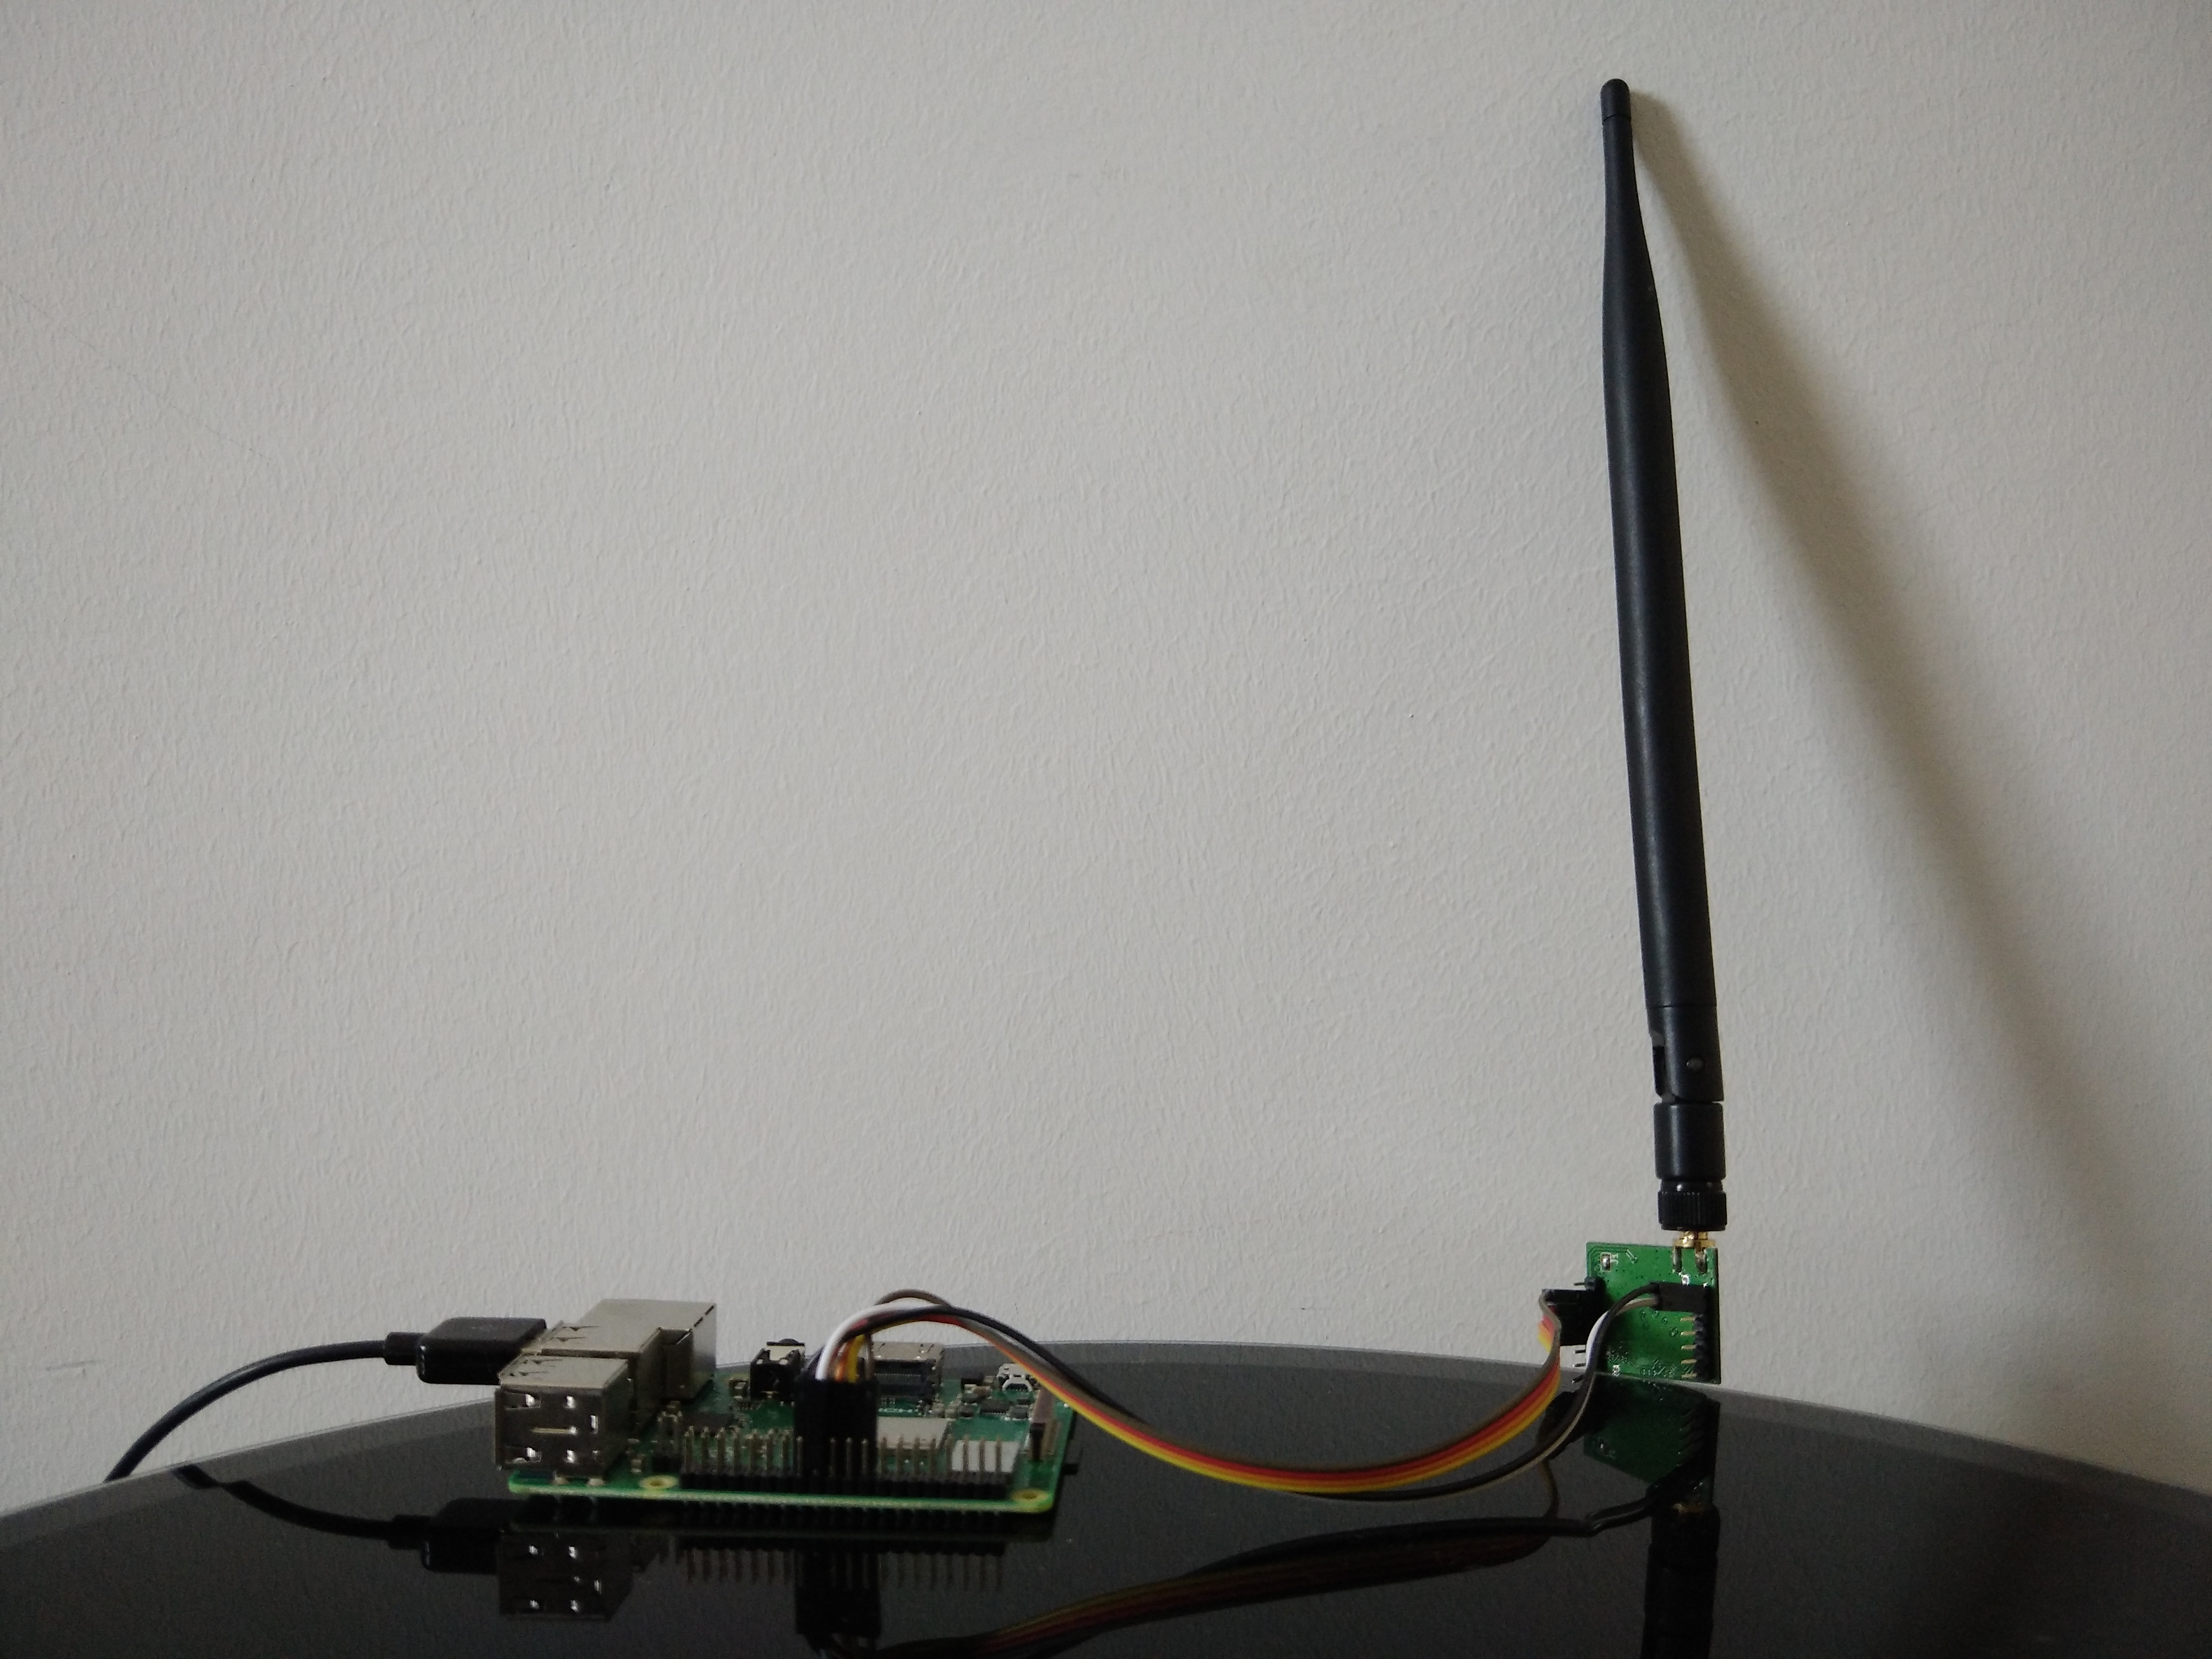
\includegraphics{gateway}} &
%\RESPATHizebox{60mm}{!}{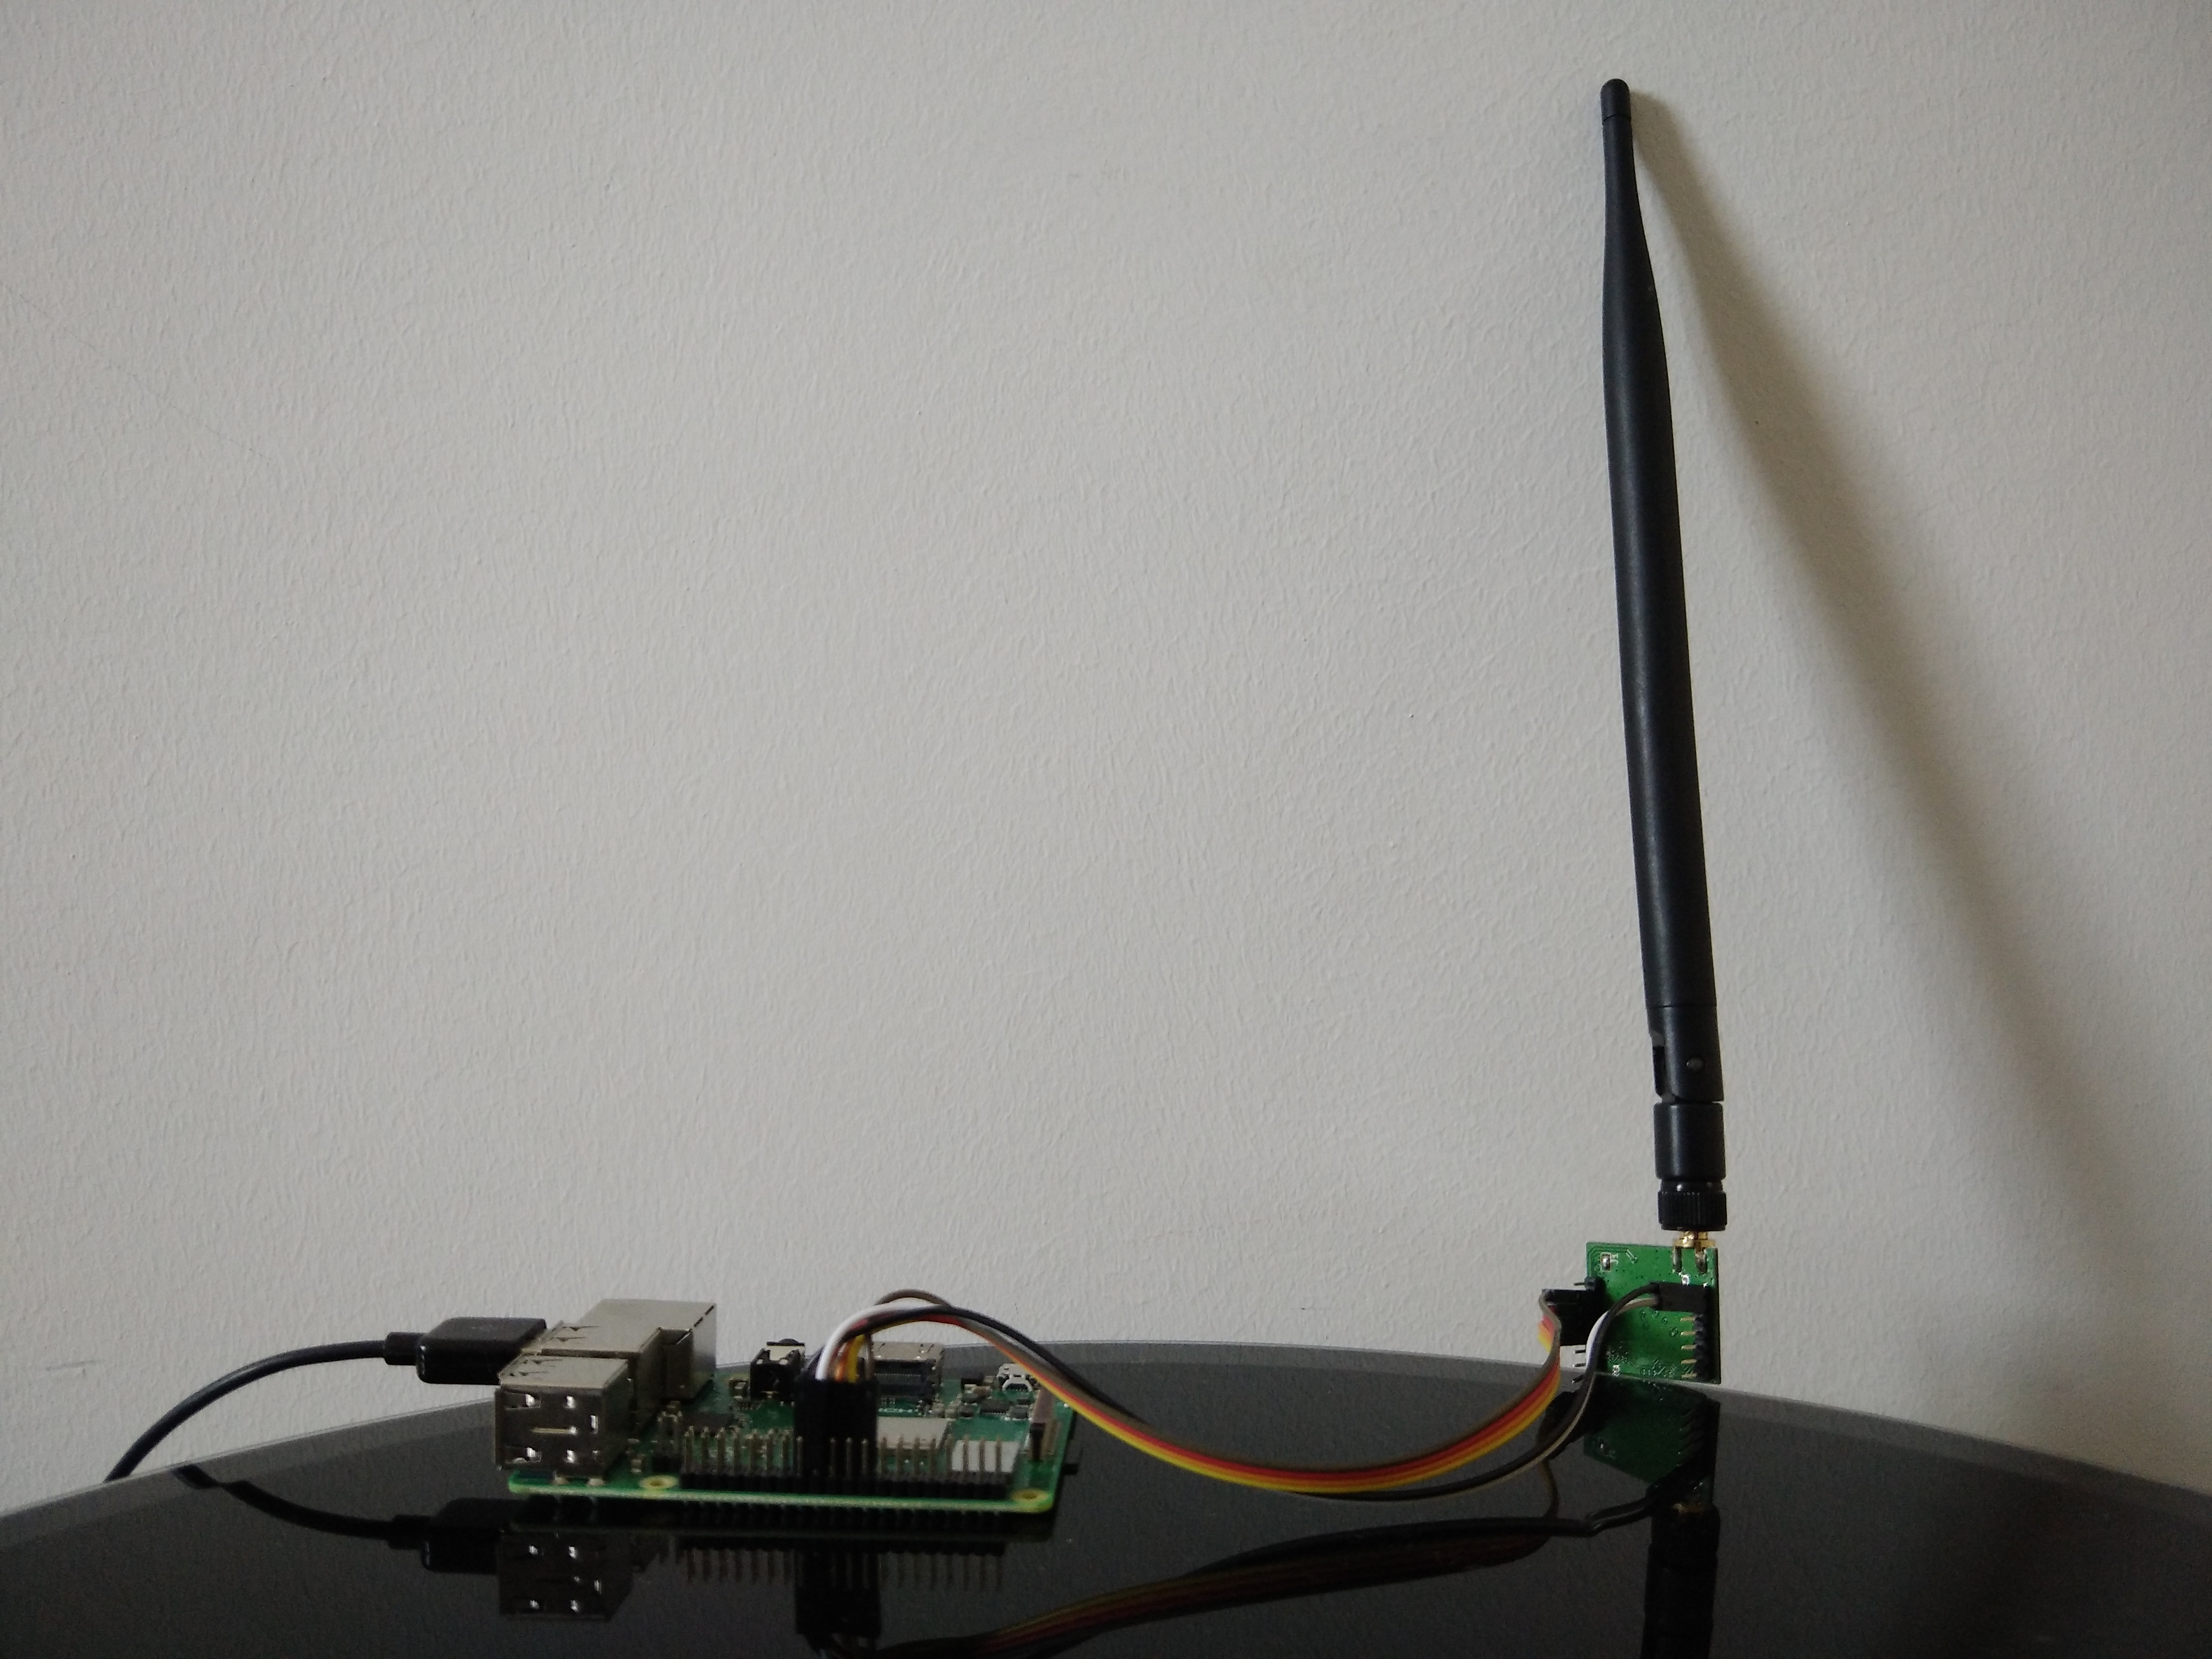
\includegraphics{gateway}} \\
%\RESPATHizebox{60mm}{!}{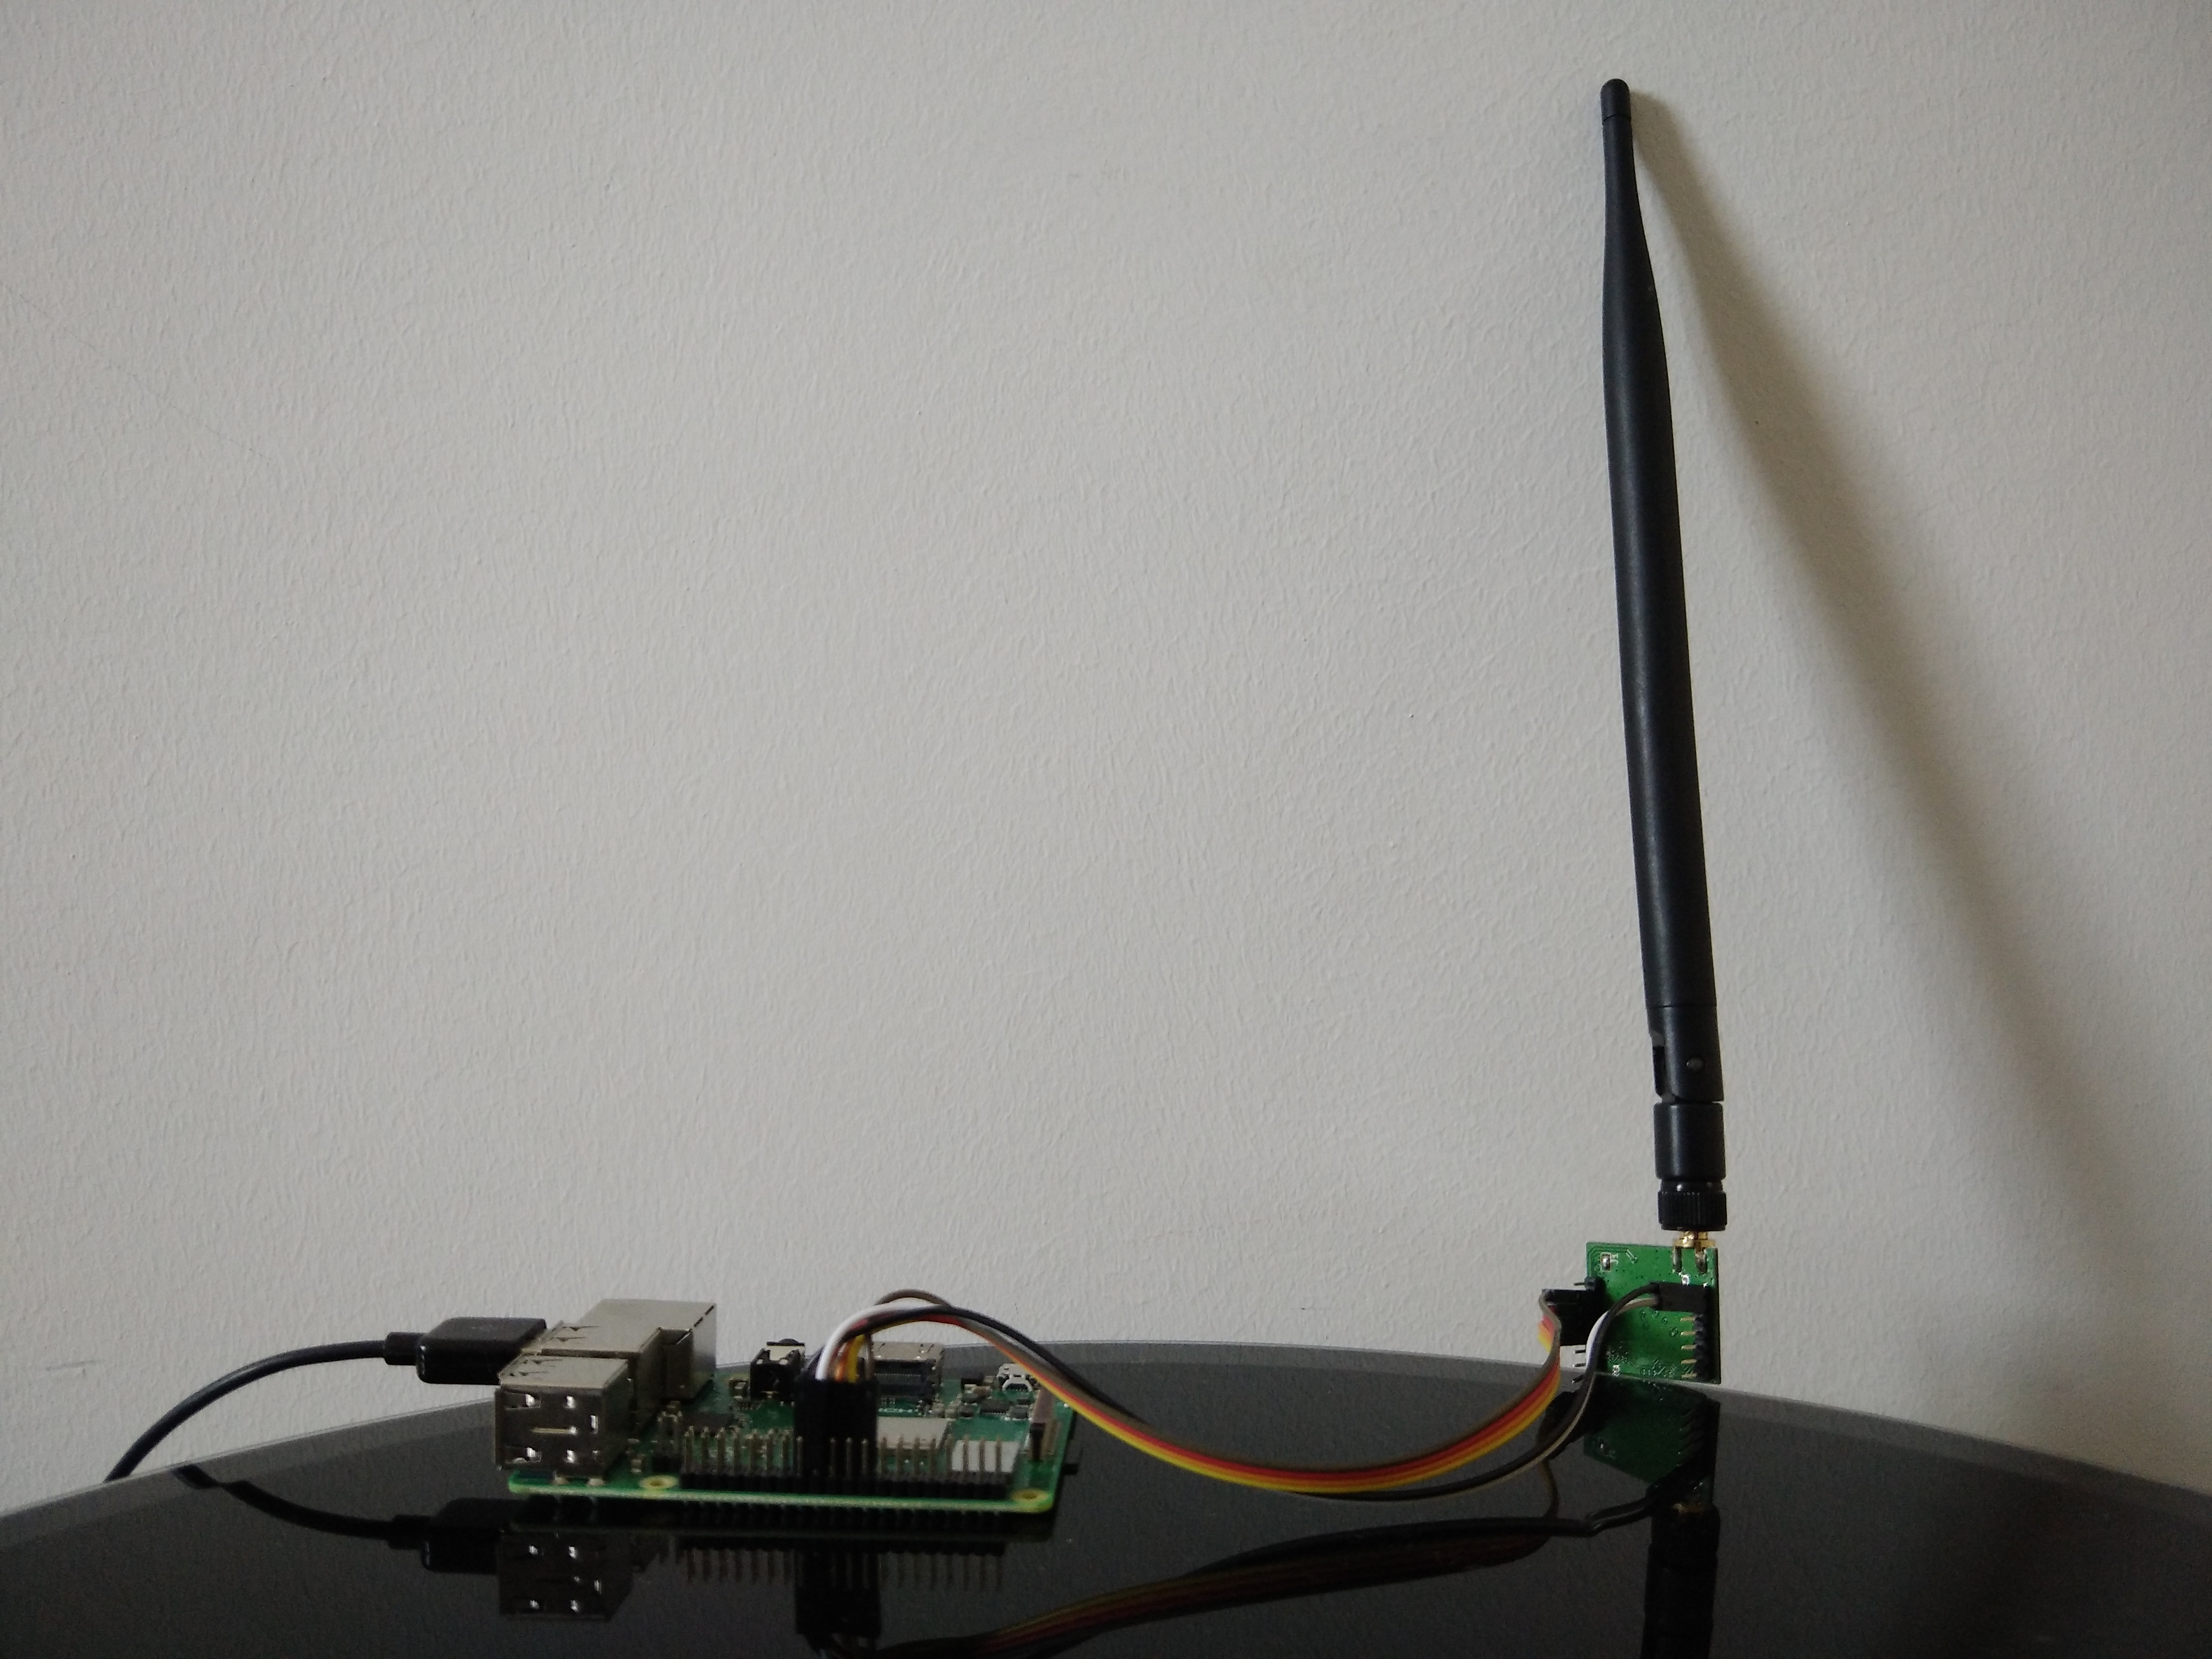
\includegraphics{gateway}} &
%\RESPATHizebox{60mm}{!}{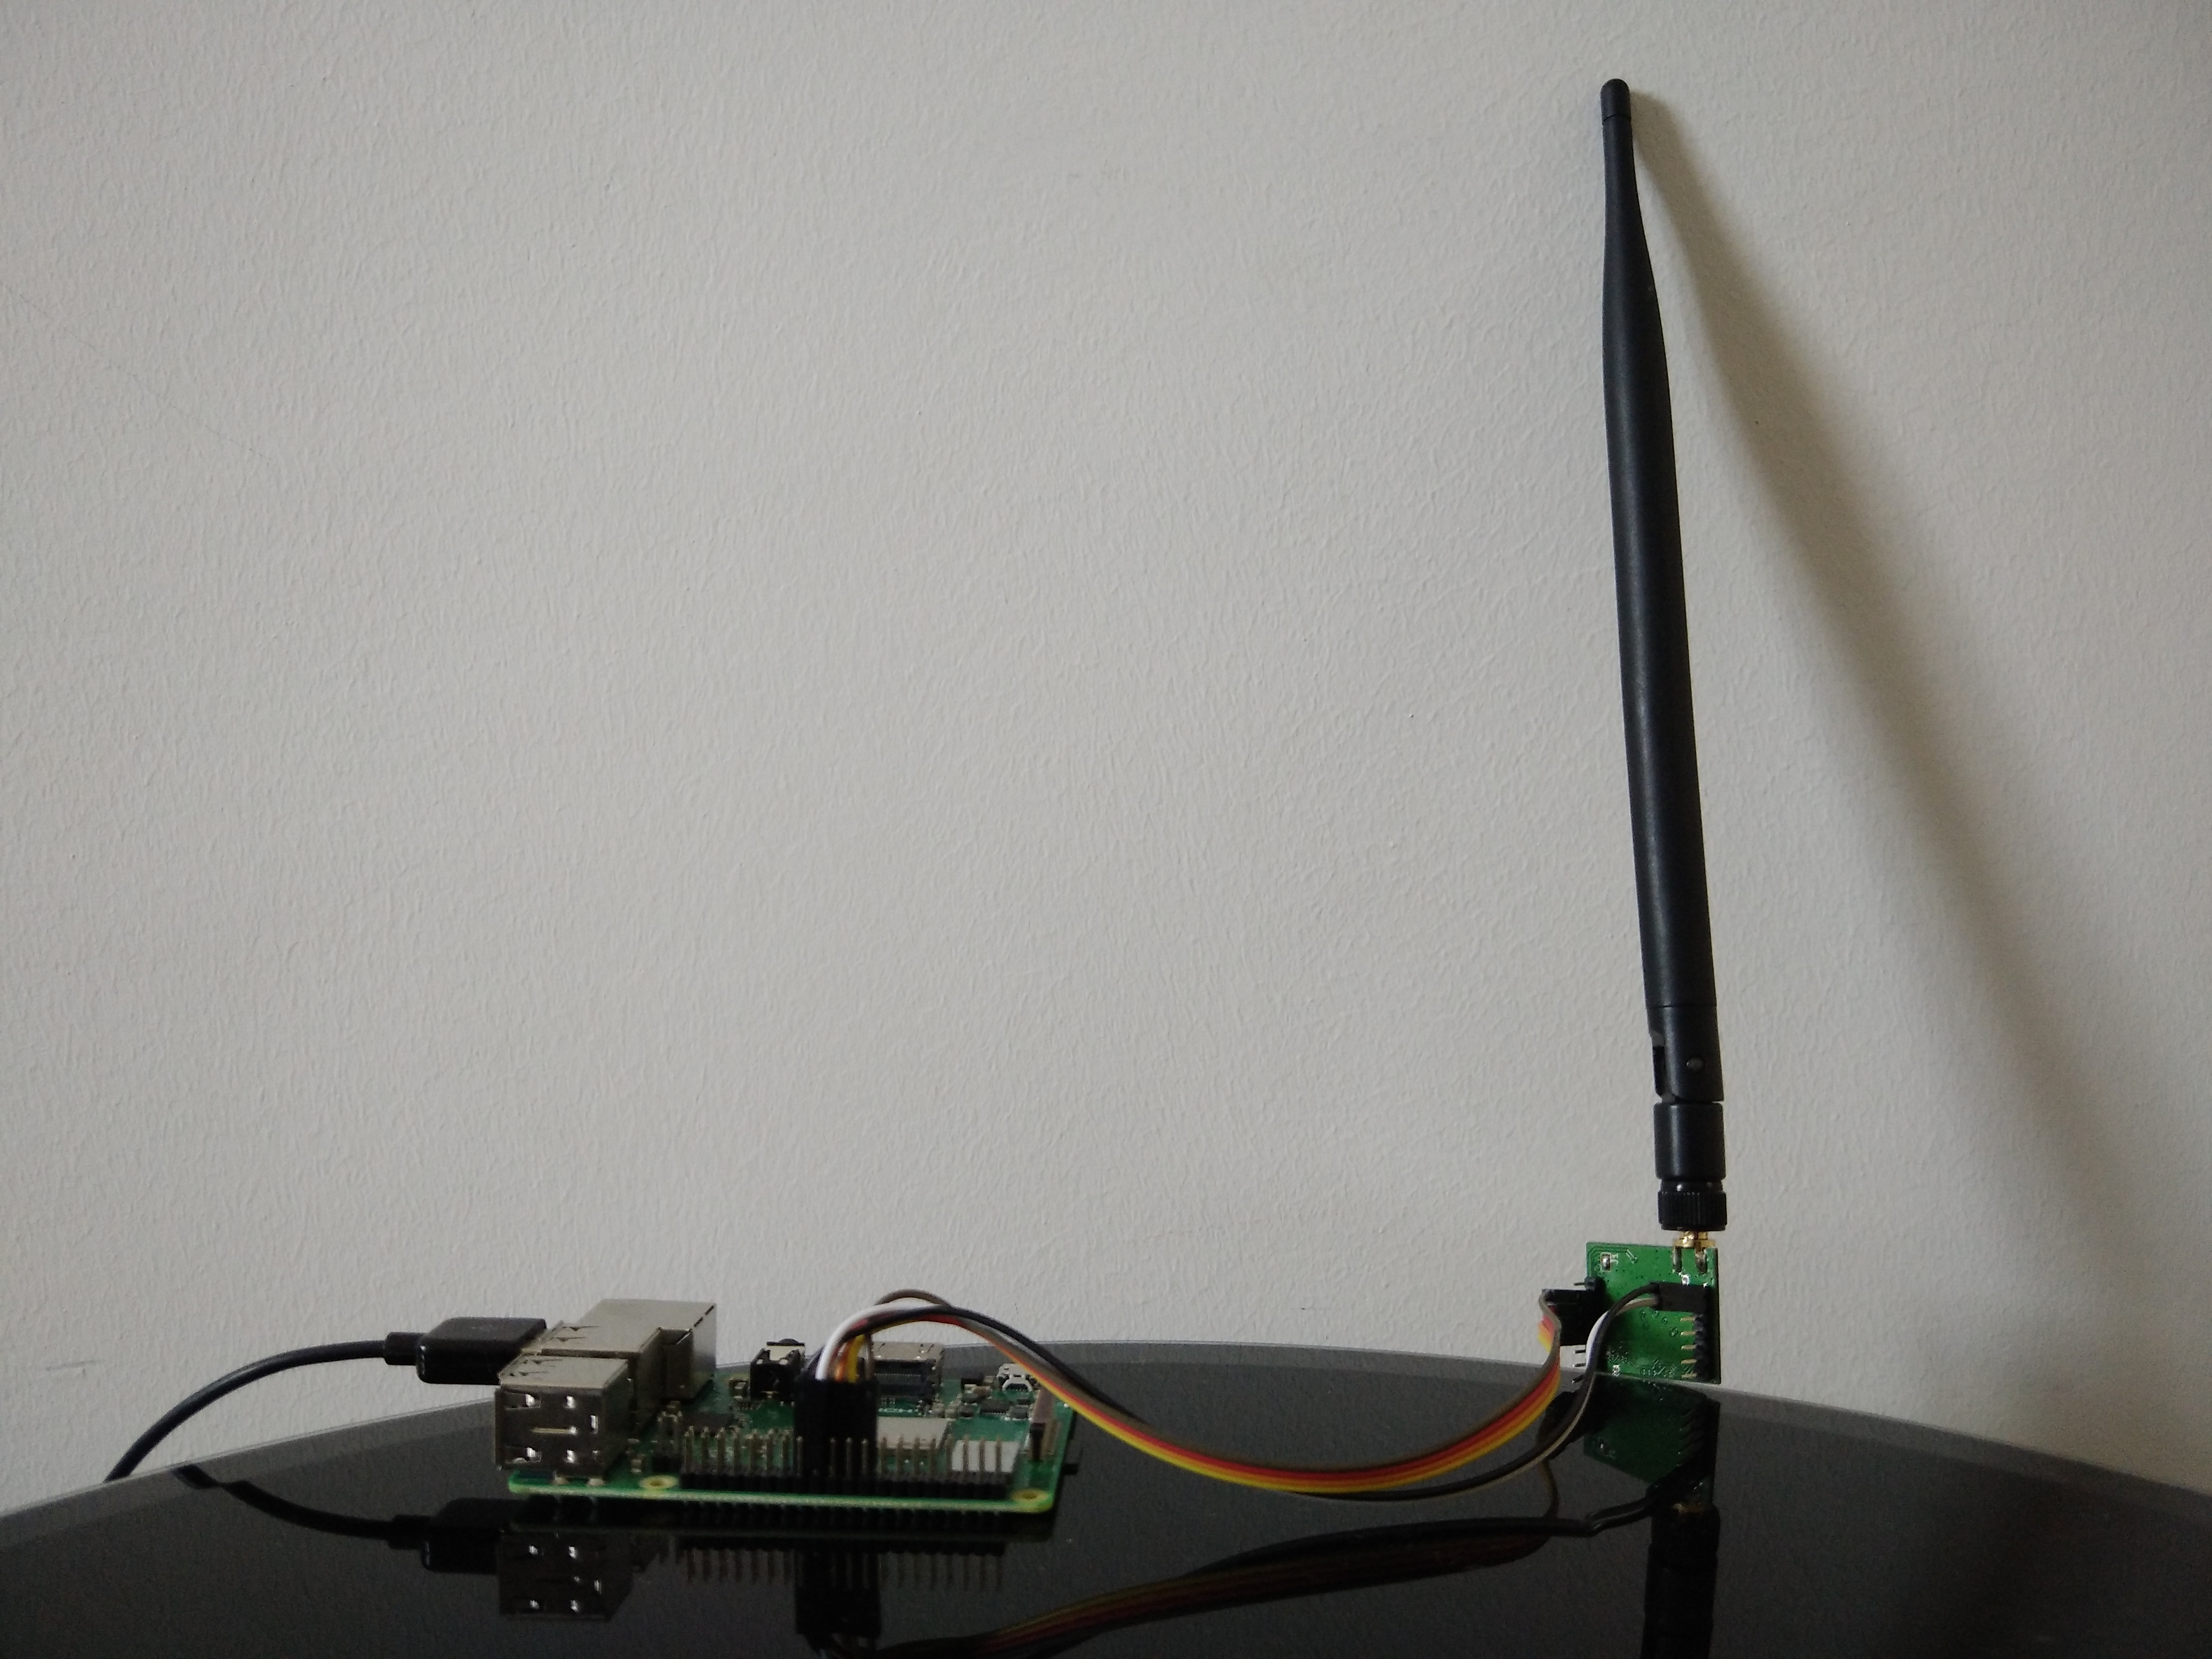
\includegraphics{gateway}} \\
%\end{tabular}
%\caption{This is sample figures.}
%\label{test4}
%\end{center}
%\end{figure}


% \documentclass[a4paper, 92pt, twoside, openright]{report}

\usepackage[top=2.5cm, bottom=2cm, left=3cm, right=2.5cm, headheight=15pt]{geometry}
\usepackage{xparse}
	\ExplSyntaxOn
		\NewDocumentCommand{\xinput}{m}{%
			\azimut_xinput:n { #1 }
		}
		\ior_new:N \g_azimut_xinput_stream
		\cs_new_protected:Nn \azimut_xinput:n{
			\ior_open:Nn \g_azimut_xinput_stream { "|ls ~ #1" }
			\ior_map_inline:Nn \g_azimut_xinput_stream { \file_input:n { \tl_trim_spaces:n {##1} } }
		}
	\ExplSyntaxOff
	
% First page %%%%%%%%%%%%%%%%%%%%%%%%%%%%%%%%%%%%%%%%%%%%%%%%%%%%%%%%%%%%%%%%%%%%%
\def\titlepage{
	\newpage
	\centering
	\linespread{1}
	\normalsize
	\vbox to \vsize\bgroup\vbox to 9in\bgroup
}
\def\endtitlepage{
	\par
	\kern 0pt
	\egroup
	\vss
	\egroup
	\cleardoublepage
}

\pagestyle{empty}
\makeatletter
	\def\@ecole{école}
	\newcommand{\ecole}[1]{\def\@ecole{#1}}

	\def\@specialite{Spécialité}
	\newcommand{\specialite}[1]{\def\@specialite{#1}}

	\def\@directeur{directeur}
	\newcommand{\directeur}[1]{\def\@directeur{#1}}

	\def\@encadrant{encadrant}
	\newcommand{\encadrant}[1]{\def\@encadrant{#1}}
	
	\def\@jurya{}{}{}
	\newcommand{\jurya}[3]{\def\@jurya{#1,	& #2	& #3\\}}
	
	\def\@juryb{}{}{}
	\newcommand{\juryb}[3]{\def\@juryb{#1,	& #2	& #3\\}}
	
	\def\@juryc{}{}{}
	\newcommand{\juryc}[3]{\def\@juryc{#1,	& #2	& #3\\}}
	
	\def\@juryd{}{}{}
	\newcommand{\juryd}[3]{\def\@juryd{#1,	& #2	& #3\\}}
	
	\def\@jurye{}{}{}
	\newcommand{\jurye}[3]{\def\@jurye{#1,	& #2	& #3\\}}
	
	\def\@juryf{}{}{}
	\newcommand{\juryf}[3]{\def\@juryf{#1,	& #2	& #3\\}}
	
	\def\@juryg{}{}{}
	\newcommand{\juryg}[3]{\def\@juryg{#1,	& #2	& #3\\}}
	
	\def\@juryh{}{}{}
	\newcommand{\juryh}[3]{\def\@juryh{#1,	& #2	& #3\\}}
	
	\def\@juryi{}{}{}
	\newcommand{\juryi}[3]{\def\@juryi{#1,	& #2	& #3\\}}
\makeatother

\newcommand\BackgroundPic{%
	\put(0,0){%
		\parbox[b][\paperheight]{\paperwidth}{%
			
\includegraphics[height=0.45\paperheight]{Bordure.png}%
			\vfill
		}
	}
}
\newcommand\EtiquetteThese{%
	\put(0,0){%
		\parbox[t][\paperheight]{\paperwidth}{%
			\hfill
			\colorbox{blue}{
				\begin{minipage}[b]{3em}
					\centering\Huge\textcolor{white}{T\\H\\E\\S\\E\\}
					\vspace{0.2cm}
				\end{minipage}
			}
		}
	}
}

\makeatletter
\newcommand{\firstpage}{
	\newgeometry{top=2.5cm, bottom=2cm, left=2cm, right=1cm}
	\AddToShipoutPicture*{\BackgroundPic}
	\AddToShipoutPicture*{\EtiquetteThese}
	\begin{titlepage}
		\centering
			
\includegraphics[width=0.2\textwidth]{upmc}
			\hfill
			
\includegraphics[width=0.2\textwidth]{sorbonne}\\
		\vspace{1cm}
			{\Large \'{E}cole doctorale 364 : Sciences Fondamentales et Appliquées}\\
		\vspace{1cm}
			{\huge {\bfseries Doctorat ParisTech}\\
		\vspace{0.5cm}
			TH\`{E}SE}\\
		\vspace{1cm}
			{\bfseries pour obtenir le grade de docteur délivré par}\\
		\vspace{1cm}
			{\huge\bfseries \@ecole}\\
		\vspace{0.5cm}
			{\Large{\bfseries Spécialité doctorale ``\@specialite''}}\\
		\vspace{2cm}
			\textit{présentée et soutenue publiquement par}\\
		\vspace{0.5cm}
			{\Large {\bfseries \@author}} \\
		\vspace{0.5cm}
			le \@date \\
		\vfill
			{\LARGE \color[rgb]{0,0,1} \bfseries{\@title}} \\
		\vfill
			Directeur de thèse : {\bfseries \@directeur}\\
			Co-encadrant de thèse : {\bfseries \@encadrant}\\
		\vfill
		\begin{tabular}{>{\bfseries}llr}
			\large Jury\\
			\@jurya
			\@juryb
			\@juryc
			\@juryd
			\@jurye
			\@juryf
			\@juryg
			\@juryh
			\@juryi
		\end{tabular}
		\vfill
	\end{titlepage}
	\restoregeometry
}
\makeatother

% Preface %%%%%%%%%%%%%%%%%%%%%%%%%%%%%%%%%%%%%%%%%%%%%%%%%%%%%%%%%%%%%%%%%%%%%%
\def\abstract{
	% \chapter*{Abstract}
	\begin{center}{
		\large\bf Abstract}
	\end{center}
	\small
	\linespread{1.5}
	\normalsize
}

\def\endabstract{
	\par
}

\newenvironment{acknowledgements}{
	\cleardoublepage
	\begin{center}{
		\large \bf Acknowledgements}
	\end{center}
	\small
	\linespread{1.5}
	\normalsize
}{\cleardoublepage}

\def\endacknowledgements{
	\par
}

\newenvironment{dedication}{
	\small
	\linespread{1.5}
	\normalsize
}{\cleardoublepage}

\def\enddedication{
	\par
}

\usepackage{setspace}
\def\preface{
	\pagenumbering{roman}
	\pagestyle{plain}
%	\doublespacing
	\chapter*{Abstract}{}
	\addcontentsline{toc}{chapter}{Abstract}
		Nowadays,
	Internet of things is witnessing a tremendous evolution due to the increasing growth in communication technologies,
	weather and environmental sensing, health care sensing.
Indeed,
	sensors are being a kind of intelligent mobile agent able to perceive its environment and transmit information to the cloud for processing,
This way of perception allow the development of several kinds of applications to enhance human capacity to understand their environment and make appropriate decision.
However,
	developing such advanced applications relies heavily on the quality of the communication between sensors and between sensors and the infrastructure,
	therefore,
	such communication can be realized only with the help of a secure data collection and efficient data treatment and analysis.

%Thematique
Data collection in a vehicular network has been always a real challenge due to the specific characteristics of these highly dynamic networks (frequent changing topology,
	vehicles speed and frequent fragmentation),
	which lead to opportunistic and non long-lasting communications.
Security,
	remains another weak aspect in these wireless networks since they are by nature vulnerable to various kinds of attacks aiming to falsify collected data and affect their integrity.
Furthermore,
	collected data are not understandable by themselves and could not be interpreted and understood if directly shown to a driver or sent to other nodes in the network.
They should be treated and analyzed to extract meaningful features and information to develop reliable applications.
In addition,
	developed applications always have different requirements regarding quality of service (QoS).
Several research investigations and projects have been conducted to overcome the aforementioned challenges.
However,
	they still did not meet perfection and suffer from some weaknesses.
For this reason,
	we focus our efforts during this thesis to develop a platform for a secure and efficient data collection and exploitation to provide vehicular network users with efficient applications to ease their travel with protected and available connectivity.
Therefore,
	we first propose a solution to deploy an optimized number of data harvesters to collect data from an urban area.
Then,
	we propose a new secure intersection based routing protocol to relay data to a destination in a secure manner based on a monitoring architecture able to detect and evict malicious vehicles.
This protocol is after that enhanced with a new intrusion detection and prevention mechanism to decrease the vulnerability window and detect attackers before they persist their attacks using Kalman filter.
In a second part of this thesis,
	we concentrate on the exploitation of collected data by developing an application able to calculate the most economic itinerary in a refined manner for drivers and fleet management companies.
This solution is based on some information that may affect fuel consumption,
	which are provided by vehicles and other sources in Internet accessible via specific APIs,
	and targets to economize money and time.
Finally,
	a spatio-temporal mechanism allowing to choose the best available communication medium is developed.
This latter is based on fuzzy logic to assess a smooth and seamless handover,
	and considers collected information from the network,
	users and applications to preserve high quality of service.





	\chapter*{Résumé}{}
		\input{00/01_2_abstract_french}

	
\includepdf[pages=1]{00/01_3_abstract_tifinagh.pdf}

	
\includepdf[pages=1]{00/01_4_abstract_arabic.pdf}

	\chapter*{Acknowledgements}{}
	\addcontentsline{toc}{chapter}{Acknowledgements}
		\input{00/02_acknowledgements}

	\chapter*{Dedication}{}
	\addcontentsline{toc}{chapter}{Dedication}
	

%\vspace*{\fill}
%\begin{center}
%To the best mother ever, my mother
%\end{center}
%\vspace*{\fill}


}

\makeatletter
\def\chapapp2{Chapter}

\def\ps@pheadings{
	\let\@mkboth\markboth
	% modifications
	\def\@oddhead{
		\protect\underline{
			\protect\makebox[\textwidth][l]
			{\sl\rightmark\hfill\rm\thepage/\pageref{pba}}
		}
	}
	\def\@oddfoot{}
	\def\@evenfoot{}
	\def\@evenhead{
		\protect\underline{
			\protect\makebox[\textwidth][l]
			{\rm\thepage\hfill\sl\leftmark}
		}
	}
	% end of modifications
	\def\chaptermark##1{
		\markboth{
			\ifnum \c@secnumdepth >\m@ne
			\chapapp2\ \thechapter. \ \fi ##1
		}{}
	}
	\def\sectionmark##1{
		\markright {
			\ifnum \c@secnumdepth >\z@
			\thesection. \ \fi ##1
		}
	}
}
\makeatother

% Body     %%%%%%%%%%%%%%%%%%%%%%%%%%%%%%%%%%%%%%%%%%%%%%%%%%%%%%%%%%%%%%%%%%%%%%
%uhead
\makeatletter
\def\chapapp2{Chapter}
\def\ps@uheadings{
	\let\@mkboth\markboth
	% modifications
	\def\@oddhead{
		\protect\underline{
			\protect\makebox[\textwidth][l]
			{\sl\rightmark\hfill\rm\thepage/\pageref{pba}}
		}
	}
	\def\@oddfoot{}
	\def\@evenfoot{}
	\def\@evenhead{
		\protect\underline{
			\protect\makebox[\textwidth][l]
			{\rm\thepage/\pageref{pba}\hfill\sl\leftmark}
		}
	}
	% end of modifications
	\def\chaptermark##1{
		\markboth{
			\ifnum \c@secnumdepth >\m@ne
			\chapapp2\ \thechapter. \ \fi ##1
		}{}
	}
	\def\sectionmark##1{
		\markright {
			\ifnum \c@secnumdepth >\z@
			\thesection. \ \fi ##1
		}
	}
}
\makeatother

\makeatletter  %to avoid error messages generated by "\@". Makes Latex treat "@" like a letter
\usepackage{epigraph}
\usepackage{setspace}
\def\body{
%		\cleardoublepage
%		\pagestyle{pheadings}
%		\listoftodos[ToDo]
%		\pagestyle{plain}
		%/
		\cleardoublepage
		\pagestyle{pheadings}
		\dominitoc
		\setcounter{tocdepth}{6}
		\tableofcontents
		\pagestyle{plain}
		%4
		\cleardoublepage
		\pagestyle{uheadings}
		\dominilot
		\listoftables
		\pagestyle{plain}
		%5
		\cleardoublepage
		\pagestyle{uheadings}
		\dominilof
		\listoffigures
		\pagestyle{plain}
		%6
		\cleardoublepage
		\pagestyle{uheadings}
		\chapter*{List of Abbreviations}
		\printacronyms[include-classes=abbrev,name=]
		\addcontentsline{toc}{chapter}{List of Abbreviations}
		\pagestyle{plain}
		%7
		\cleardoublepage
		\pagestyle{uheadings}
		\chapter*{List of Nomenclatures}
		\printacronyms[include-classes=nomencl,name=]
		\addcontentsline{toc}{chapter}{List of Nomenclatures}
		\pagestyle{plain}
		%8
		\cleardoublepage
		\pagestyle{uheadings}
		\chapter*{List of Publications}
		\epigraph{''There's no absolutely reliable way to achieve a great citation. However, hardworking could be fruitful'' -  Eraldo Banovac}{}
		\addcontentsline{toc}{chapter}{List of Publications}
		\section*{International Conferences}

\section*{National Conferences}

\section*{Journals}

\section*{Survey}

		\pagestyle{plain}

		\cleardoublepage
		\pagestyle{uheadings}
		\pagenumbering{arabic}
		\setcounter{mtc}{9}
		\setcounter{secnumdepth}{6}
		%\setlength{\parskip}{3ex plus 0.5ex minus 0.2ex}
}
\makeatother	%to avoid error messages generated by "\@". Makes Latex treat "@" like a letter

% Appendix %%%%%%%%%%%%%%%%%%%%%%%%%%%%%%%%%%%%%%%%%%%%%%%%%%%%%%%%%%%%%%%%%%%%%%
\def\Appendix{
	\oldlabel{pba}
	\appendix
	\pagestyle{plain}
}


% Section %%%%%%%%%%%%%%%%%%%%%%%%%%%%%%%%%%%%%%%%%%%%%%%%%%%%%%%%%%%%%%%%%%%%%
\usepackage[section]{placeins}	% Place un FloatBarrier à chaque nouvelle section
\usepackage[font={small}]{caption}
\usepackage{minitoc}		% Mini table des matières, en français
	\setcounter{minitocdepth}{4}
	\setlength{\mtcindent}{12pt}
	\renewcommand{\mtcfont}{\small\rm}
	\renewcommand{\mtcSfont}{\small\bf}
\usepackage[notbib]{tocbibind}		% Ajoute les Tables	des Matières/Figures/Tableaux à la table des matières


% Chapter %%%%%%%%%%%%%%%%%%%%%%%%%%%%%%%%%%%%%%%%%%%%%%%%%%%%%%%%%%%%%%%%%%%%%
\usepackage{titlesec, blindtext}
	\usepackage[titles]{tocloft}
	\newlistentry[subparagraph]{subsubparagraph}{toc}{5}
	%\newcounter{subsubparagraph}
	\titleclass{\subsubparagraph}{straight}[\subparagraph]
	\renewcommand{\theparagraph}{\arabic{paragraph})}
	\renewcommand{\thesubparagraph}{\arabic{paragraph}.\arabic{subparagraph})}
	\renewcommand{\thesubsubparagraph}{\Alph{subsubparagraph})}
	\titleformat{\chapter}[hang]
			{\Huge\bfseries}
			{\violet{\thechapter\hspace{20pt}|\hspace{20pt}}}{0pt}
			{\Huge\bfseries}
	\titleformat*{\chapter}{\normalfont\huge\bfseries\color{violet}}
	\titleformat*{\section}{\normalfont\Large\bfseries\color{violet}}
	\titleformat*{\subsection}{\normalfont\large\bfseries\color{violet}}
	\titleformat*{\subsubsection}{\normalfont\bfseries\color{violet}}
	\titleformat*{\paragraph}{\normalfont\bfseries\color{violet}}
	\titleformat*{\subparagraph}{\normalfont\color{violet}}
	\titleformat{\subsubparagraph}[runin]{\normalfont\normalsize\bfseries}{\thesubsubparagraph}{1em}{}
	\titleformat*{\subsubparagraph}{\normalfont\color{violet}}

\makeatletter
	\let\stdchapter\chapter
	\renewcommand*\chapter{%
		\removelabelprefix
		\addlabelprefix{\thechapter}
		\@ifstar{\starchapter}{\@dblarg\nostarchapter}}
	\newcommand*\starchapter[1]{
		\stdchapter*{#1}
	}
	\def\nostarchapter[#1]#2{
		\StrCount{#1}{:}[\nbmatch]%
		\StrCut[\nbmatch]{#1}{:}\strchapfirst\strchapsecond%
		\stdchapter{#2}
		%\epigraph{\strchapsecond}
		\minitoc
		\xinput{#1*/0*}
	}
\makeatother


% Table of content %%%%%%%%%%%%%%%%%%%%%%%%%%%%%%%%%%%%%%%%%%%%%%%%%%%%%%%%%%%%%%%%%%%%%
\titlespacing*{\subsubparagraph}{\parindent}{1ex plus .5ex minus .5ex}{1em}
	\cftsetindents{part}           {00em}{1em}
	\cftsetindents{chapter}        {00em}{2em}
	\cftsetindents{section}        {00em}{3em}
	\cftsetindents{subsection}     {00em}{4em}
	\cftsetindents{subsubsection}  {00em}{5em}
	\cftsetindents{paragraph}      {05em}{1.5em}
	\cftsetindents{subparagraph}   {05em}{2.5em}
	\cftsetindents{subsubparagraph}{7.5em}{1.5em}


% Citation %%%%%%%%%%%%%%%%%%%%%%%%%%%%%%%%%%%%%%%%%%%%%%%%%%%%%%%%%%%%%%%%%%%%%
\usepackage{epigraph}
	\setlength\epigraphwidth{8cm}
	\setlength\epigraphrule{0pt}
	\renewcommand\textflush{flushright}
	\renewcommand\epigraphsize{\normalsize\itshape}


\xinput{00/00_firstpage}


\renewcommand\twocolumn{}


\def\Keywords#1{

}
